% !TEX encoding = UTF-8 Unicode
\documentclass[12pt,oneside]{book}

\usepackage{fontspec}
\defaultfontfeatures{Mapping=tex-text,Scale=MatchLowercase}
\setmainfont{Lato}
%\setmonofont{Fira Mono}

\pagestyle{plain}
\usepackage{setspace}
\usepackage{enumitem}

% make block quotes fancy
\usepackage{csquotes}
\usepackage[onehalfspacing]{setspace}
\makeatletter
\newcommand*{\singlespacingNoVspace}{%
  \setstretch{\setspace@singlespace}}
\makeatother
\newenvironment{singlequote}
  {\quote\singlespacingNoVspace}
  {\endquote}

\SetBlockEnvironment{singlequote}

\usepackage{geometry}
%\geometry{letterpaper}
\geometry{a4paper}
\usepackage{graphicx}
\usepackage{epigraph}
\setlength\epigraphwidth{.45\textwidth}

%% For highlight ranges of text marked with inspector comments
\usepackage{soul}

\usepackage{xcolor}
\usepackage[
    colorlinks=true,
    urlcolor=blue,
    linkcolor=blue,
    citecolor=blue,
    filecolor=blue,
]{hyperref}
\usepackage{memhfixc}
\usepackage{mdframed}

\setcounter{page}{1}
\pagenumbering{roman}

\renewcommand*\contentsname{contents}

\begin{document}

\begin{titlepage}
    \begin{center}
        \vspace*{1cm}
            
        \huge{
        \textbf{a practical guide to \\research software project estimation}\\}
        \hfill \break \fill \break
        \small{20220525 v1.0}
        \vfill
        \large{
        \textbf{Chase Million}\\
        Million Concepts\\}

    \end{center}
\end{titlepage}

%\maketitle
\clearpage


\tableofcontents

% \listoffigures
% \listoftables

%\section*{Foreward}

\newpage
\setcounter{page}{1}
\pagenumbering{arabic}

\mainmatter
\setstretch{1.12}
\addcontentsline{toc}{chapter}{introduction}
\chapter*{introduction}

Most texts on software engineering or software project management assume applications in commercial or business settings. While there are some texts on topics related to the use of specific programming languages, techniques, and paradigms in research---like ``cookbooks'' for efficiently implementing numerical algorithms---there are few that address broader software systems engineering and project management in research contexts.\footnote{
The most famous and impactful of the ``cookbook'' genre is certainly “Numerical Recipes,” which---although it has had a profound influence on a wider range of disciplines---was co-written by a computational physicist working on difficult models of computational relativity, Saul Teukolsky. I also very briefly worked for him as an undergraduate. I think I lasted less than a week. As I remember it, my main reason for quitting was that the job was mostly programming and I did not want to be a ``code monkey.'' That seems to have happened anyway. Oops.}

As a consequence, the available references on these topics focus on situations that many scientists will never encounter in their careers, including (relative to industry) complicated org charts, difficult procurement processes, strict contract terms and deliverables, and large budgets. Software development standards
%\footnote{e.g. ISO/IEC/IEEE 12207}
and ``best practices'' can be opaque to scientists who do not have engineering backgrounds. They can often seem irrelevant even to those who do.

The dearth of information and training in project management frequently results in poorly-planned, inadequately-supported, incompletely-executed, or shoddy research software. This is of course not a problem unique to research. Software development suffers from being undersupported in many fields and organizations. This may be because software is intangible; perhaps its ethereal nature makes it feel less valuable or less difficult to produce, that it should therefore demand fewer resources. This bias is not limited to people who do not themselves produce software; software developers tend to undervalue their own efforts and routinely underestimate the amount of work it will take them to make good software.

Within the academy, I suspect that the problem is exacerbated by the fact that very few of the people who establish the budgets allocated to the software portions of research efforts---faculty and other research scientists at universities---have any background in systems engineering or software project management, and few of them are ``programmers'' except incidentally to their research pursuits (e.g. using a programming environment as a powerful graphing calculator). Not only do they not know what amount of support would be reasonable for any particular software project, but they do not know how to go about figuring it out. The people responsible for judging requests for support---proposal reviewers and agency program officers---also do not typically have the backgrounds that would enable them to make sound recommendations or judgements. Many projects that have allocated insufficient support for software tasks are therefore, nonetheless, funded and attempted, as everyone involved was ill-equipped to discover that too few resources were requested.\footnote{
Many of these projects are nonetheless successful, to be fair. But it is often a much shallower success than it could have been, and is achieved only via sacrifice and heroism.}

One very good reason to do a better job estimating research software tasks is that it will ensure that sufficient support is available to achieve the research objectives. This is good for the research, obviously. But it also has clear benefits to the staff and researchers, who will know that they are being properly supported in their work and will not labor under the nagging, frustrating, demoralizing suspicion that they've been set up to fail.

Well-scoped research software projects are more likely to generate better research software that is more in line with the needs of researchers, better validated, sustainable, and cleaner. This benefits the scientific ecosystem as a whole; it provides better documentation of the analyses performed, improves reproducibility, and can reduce duplicated research effort within and between research groups. Increasingly, the most accurate documentation of how research was conducted exists in code. This is almost always the case for physical simulations and numerical analysis of observational data. It is also generally true for fields in which the majority of observational data arrives to researchers in digital form---which means most fields in the present day.

Another very good reason to do a better job estimating research software tasks---or research projects more broadly---is that it will almost certainly generate better research proposals, which has at least some correlation with winning research grants. I have reviewed and---in my shamefully naive past---written many research proposals in which the ``work plan'' occupied no more than 2 of 15 pages. A typical research grant in my field is on the order of \$150-250k per year over 3 years, so it seems curious (and often comes up for discussion in proposal reviews!) that someone would ask for access to so much money with minimal explanation for how it will be spent. I think that the reason that most people don't include more description of ``work plan'' is that they don't have a work plan to describe. They don't have that plan because the standard scientific training regiment does not include even introductory information about project management or systems engineering, the domains that encompass project scoping and estimation.\footnote{
Research endeavors, even those with no obvious “engineering” component, are systems engineering problems. There’s probably more to be gleaned from this observation, but it’s outside of the scope of this text.}

I have been part of many proposals for which the PI first declared a bottom-line budget for the project---before writing the proposal!---based upon historical averages for the program, and then wrote the proposal by fiddling with the budget particulars to fit within this cap, giving almost no regard for the scope of the work. This is the project planning equivalent of Escher's hand drawing itself. I believe that an easily-understood method to generate software project estimates that are both reasonable and sufficient can help scientists formulate better proposals for research projects that include substantial software engineering elements, and that this will consequently improve the overall quality of research software. This document is my attempt to quickly convey such a method.

The primary audience for this document is people who are conceiving of and writing proposals for original research projects. In terms of traditional academic career paths, this would tend to include most faculty, many post-docs, and some graduate students. Candidate Principal Investigators will learn how to scope, estimate, and plan an effort so that they can compose a plausible work plan and a budget that requests reasonable and sufficient resources for the project. A secondary audience is anybody who is taking primary ownership of portions of a research software development effort, even if that effort is already funded or underway. This might include any of the above categories and also students, research staff, or technical staff. This cohort can feel free to disregard many portions of the text that deal directly with proposal preparation.

\newpage
\addcontentsline{toc}{section}{summary of methodology}
\section*{summary of methodology}

The core approach to estimation that I'll outline is known as ``decomposition.'' In summary: take a project for which it is difficult to make an estimate, break it into smaller tasks, and then make estimates for those tasks. This is effective because it is easier to make estimates for small things than big ones, and the accumulated errors in estimating the smaller tasks will tend to average out, especially if you can moderate the impulse to systematically underestimate. As a precursor to generating the estimate, make sure that you understand the goals and constraints of the project (i.e. define its scope and requirements), so that you can be certain that you are generating an estimate for the correct project. The quality / utility of your estimate is absolutely limited by the accuracy and completeness of your scope and requirements, so I will describe how to generate those first. Then I will briefly describe how to turn an estimate into a plan or schedule and integrate these into your research proposal.

This method is best-suited to the estimation of small research software projects. What I mean by ``small'' is that the main project team is about five people or fewer; what I mean by ``research'' is that the primary objective of the project is to produce new knowledge about the world (as opposed to other common objectives like building a product, streamlining a process, or solving a technical problem---although those things might happen incidentally). This method is also well-suited to the estimation of research projects, generally, whether or not they contain significant software components. I need to specify that this is a method for projects that are ``small'' and ``research'' because most existing estimation methodologies are not very useful under these conditions, and we will therefore save ourselves the trouble of reviewing them. The estimation strategies that work best under these conditions are also, in my opinion, simple enough to be used by researchers without requiring them to become experts in systems engineering or project management.

Despite its focus, I believe this method is also suitable as a first-pass estimation methodology for \emph{nearly any project of any type or scale}. (Do you want to know how much time and money it will take you to build a bike shed? You could do worse than to apply this approach.\footnote{It's the staff bike shed at a new nuclear power plant. This is possibly irrelevant.}) However, larger projects and non-software projects and non-research projects have better estimation methodologies that can be brought to bear. Note that ``better'' tracks pretty well with ``more complex,'' up to the point where you might want to consider hiring or collaborating with someone with a solid background in project estimation in the relevant domain. Do not use the basic approach that I lay out here to generate an estimate for your fusion reactor project or space mission! But you can maybe use it in the earliest phases of planning to decide---to an order of magnitude---what amount of resources you might need to pull those things off.

You might also find this text useful for getting a general sense of the workflow and basic principles and terms of project estimation. Note, however, that I've taken quite a bit of creative license with terminology. My definitions and usages of key jargon like ``Concept of Operations,'' ``stakeholder,'' and even ``project management'' are sloppy, although more than precise enough for my purposes.

This text draws heavily on prior literature related to software project management and software project estimation, in particular ``Software Estimation: Demystifying the Black Art'' (DtBA) by Steve McConnell, ``Software Estimation Without Guessing: Effective Planning in an Imperfect World'' (SEWG) by George Dinwiddle, and ``The Project Manager's Guide to Software Engineering's Best Practices'' (TPMG) by Mark J Christensen and Richard H. Thayer. I suggest that anybody who spends a lot of time writing software for work should read these books, and I will refer to them by their acronyms later. If you are already deeply familiar with their contents, this text will probably not contain a lot of information that is new to you. I have tried to quote from and credit these works extensively, but I almost certainly missed something. If an idea appears here that also appears in one of those, all of the credit goes to those authors. Similarly, any errors are my own. Additional citations appear throughout, usually in footnotes. I believe that my primary innovation with this text has been to reframe prior work for the context of research software development. This mostly involved stripping away a lot of information that is irrelevant in many research software development contexts.

\newpage
\addcontentsline{toc}{section}{notes and limitations}
\section*{notes and limitations}
\label{scrivauto:8}

I will make reference to methods of research funding or support that only apply to academic researchers based in the United States and funded by the U.S. Federal Government via agencies like NSF, DOE, and NASA. I won't specifically note these as assumptions, because I don't know enough about funding approaches around the world to know when the U.S. system is different enough to matter. Furthermore, the vast majority of my personal experience is with projects funded through NASA, so some of my observations may be particular to the culture or procedures of that agency. For context, the types of grants that fund many researchers in this domain are called Research and Analysis (R\&A) grants; these are PI-led projects that typically have three-year terms to support a focused, hypothesis-driven investigation by a small team. In the areas of research that I have experience, there is no real opportunity to receive substantial funding from industry or other NGOs, so I've given that no consideration. If I say something that sounds like it doesn't apply to your situation, it probably doesn't, and I hope that there is enough else in here for the effort of reading this to be worthwhile for you.

All of this material should be considered \emph{caveat emptor} and YMMV. This document accurately represents my views at the time of writing. I believe that most of it is correct, that some of it is useful, and a little bit of it is interesting. But I am unlikely to be the most qualified person in the world to write this.\footnote{
Almost nobody is ever the most qualified to do anything, especially if it's interesting.}
I've written this text with my own employees and mentees in mind. If I had students, this would be the information that I would want to give them to try to maximize their chance of success and minimize unnecessary failures. I hope it's useful to you. But I am wrong about nearly everything, constantly! So you may feel free to assume that I am wrong about everything here, too.  (You don't need to tell me about it, though.)

\newpage
\addcontentsline{toc}{section}{what is an estimate?}
\section*{what is an estimate?}
\label{scrivauto:9}

Many people think that the main point of an estimate is to figure out how long something will take. Inexperienced managers or PIs who ask for estimates often think that this is what they want. Unfortunately, anyone who wants to know how long a research project will take will almost certainly be disappointed. This \emph{expectation value} is one of the most difficult things to estimate---and, in my opinion, one of the least useful. Accurate estimates---within perhaps 30\%---are extremely difficult even for expert estimators in fields like business development that often produce mountains of historical data on which to base their calculations.\footnote{And management processes and controls to constrain project costs, etc. Because it's always possible to spend more than your estimate, and you need good, active management to keep the project on track, even if the estimate is ``perfect.''} The pursuit of an accurate estimate for an original research project is foolhardy.

I think that what people most often really want when they ask for an estimate is the envelope of viability. First, they want a lower bound, meaning the minimum amount of resources or time that a project must take. This establishes the feasibility threshold of the project, because if it will take more time or resources than are available, it would be a wasted effort to undertake it. Second, they want to know what amount of time and resources provides a reasonably good guarantee of project success. This ``upper bound'' provides a reasonable budget or lead time request that minimizes the chance of cost overruns or project failure; it forms the basis for a research proposal budget, for example. And if it is larger than the allowable budget or longer than the allowable time, then there is probably an increased risk of project failure.

The method I describe in this document will help you find these bounds. You will first estimate the minimum amount of person-hours necessary to carry out a task under the best possible circumstances, then estimate what person-hours are sufficient and reasonable to carry out the project with good confidence of success. Helpfully, in this context, we can treat time (in the sense of work hours) as a direct proxy for money. This is because costs of research software projects tend to be dominated by personnel expenses; in my experience, they often eclipse other direct costs by at least two orders of magnitude.\footnote{
``Direct costs'' refers to expenses that can be attributed one-to-one to this project, like salaries for people working on this project, conference or field work travel in support of this project, or the cost of computer hardware purchased to support only this project (and no other). ``Indirect costs''---sometimes treated synonymously with ``institutional overhead''---are intended to cover expenses that cannot easily be attributed to any specific project, like rent, utilities, insurance, general use computer equipment, etc. Indirect costs are often calculated as a flat percentage of direct costs; they can be the same order of magnitude as personnel costs but scale directly with other project costs and do not need to be treated separately.}
Because work effort in research is not always compensated,\footnote{
I'm not making a normative statement here; just describing reality. For example, a common policy by grant-providing agencies is that grant funds cannot be used in the preparation of proposals. Therefore preparation of proposals, which often must contain a measure of ``research,'' is done on spec.}
and because there can be other costs to a research project---compute costs, travel, publications, etc.---I will also refer to the set of these as project ``resources.''

Also helpfully, an estimate of the person-hours necessary to perform your project's component tasks is a natural precursor to a ``plan,'' which is to say a schedule of work effort over calendar time. The required person-hours and calendar time are different because a variety of inefficiencies and bottlenecks exist in any project; for example the staff might not be available to work full time, or the project may have to wait on a critical input to be created or delivered. A good estimate and plan will help you convince yourself and others that your project is feasible and that the amount of money you have requested is sufficient to support it to a successful conclusion.\footnote{
The project might still fail, of course. But let’s try to make sure that predictable ``lack of funds'' or ``lack of time'' or other consequences of poor planning are not the cause!}
No one wants to fund doomed projects. No one wants to work on them, either! And when your well-planned project is awarded funding, you and your colleagues can proceed with confidence that you haven't set yourselves up for failure.

\newpage
\addcontentsline{toc}{section}{the basic idea}
\section*{the basic idea}

\epigraph{Just remember the three R's: \\ remove, replace, and \emph{reseal}.}{[redacted]}

Here is a complete summary of the project estimation method covered in this document. You can use this as a quick reference later. If it looks to you like this is all stuff you already know or don't care to know, you can stop now and go read something else.\footnote{I recommend \emph{Moby-Dick; or, The Whale} by Herman Melville or \emph{The Golem} by Collins and Pinch.}

\begin{enumerate}[wide, labelwidth=!, labelindent=0pt, font=\bfseries]
\item Identify project stakeholders.
\item Generate a top-level summary of the project. Define the project objectives clearly, in plain language, that all stakeholders agree on. This is called the Vision \& Scope.
\item Document the current approach to solving this problem, the functionality of the new system, and any major constraints that it must operate under from the perspective of the end users. This is called the Concept of Operations.
\item Translate the desired functionality and constraints into a number of requirements, such that if all requirements are met, the desired functionality will exist. This is called the Requirements Specification.
\item Describe an approach to meeting the requirements by performing a number of tasks, each one of which you can conceive of accomplishing successfully. This is called the Work Breakdown Structure.
\item[(Optional)] Generate a map between requirements and tasks. This is called a Requirements Traceability Matrix.
\item[6a.] Make an initial estimate of the effort of each task, in terms of hours of effort. The sum of your initial estimates forms the lower bound of your project estimate. This is the minimum amount of work effort required to achieve the project objectives, in the best possible case. If this corresponds to more time or money than is available, then the project is not feasible, and you should not undertake it as scoped.
\item[6b.] Make an estimate of your confidence in the effort of each task, by assigning it a number from [1.2, 2, 3, 4], where 1.2 is the highest level of confidence and 4 is the lowest level of confidence.\footnote{The highest level of confidence scales your estimate up by 20\% because even your most confident estimate is likely to be an underestimate. More on this later.} This should be based on your experience having done similar work in the past and the risk of unknown factors that can only be resolved after work has started. The sum of the pairwise products of your initial estimates and their confidence factors is the estimate of the amount of work effort necessary to guarantee project success with high confidence (aka the Project Estimate).
\item[6c.] Your request for resources to support this project (e.g. in a proposal budget) should be based on this final number. If this corresponds to more time or money than is available, then the risk of project failure is correspondingly higher. You should assess whether this risk of project failure is acceptable. If it is not, return to the beginning and try to be less ambitious. Under no circumstances should you simply adjust the estimate downward to a resource limit!
\end{enumerate}

\newpage
\addcontentsline{toc}{section}{convenient properties of research software}
\section*{convenient properties of research software}
\label{scrivauto:11}

Research software projects have several properties that help constrain the range of project management and estimation strategies that can and should be brought to bear. These include:\
\begin{itemize}[wide, labelwidth=!, labelindent=0pt, font=\bfseries]
\item The work is exploratory and novel. By definition, there is little historical information about similar work that can be used as the basis for an estimate. Many business models involve cranking out copies or near copies of the same type of thing---like a website or a car---and the record of how long that takes can form the basis of an estimate; but researchers on the cutting edge don't have this luxury or ability.
\item Project budgets are strictly defined at the outset. It is unusual for research and analysis (R\&A) projects to be given additional funds (so-called ``costed extensions'') after the initial award is made. This means that the budgets requested must be sufficient to assure success. This is in contrast to many business contexts in which project sponsors (e.g. business managers or clients) often want estimates that are as close to the most likely actual cost of the project as possible (the ``expectation value'') and will choose to either increase the allocation of support or not if this estimate is exceeded.\footnote{When projects exceed allocated budgets or resources in industry or commercial settings, it is common for the project teams to ask their managers or clients for additional money to complete the desired work. This can, in fact, be one possible strategy to constrain the overall project costs.}
\item Project timelines are not very strict. ``No-cost extensions''---by which the project completion date is pushed back but no additional funds are allocated---are common. This means that estimates of calendar time to complete a project are less important than estimates of total resources / personnel time / money required to complete the project. The due date should also be fluid, so that you can take more time if you need to. This gives you the flexibility that you will need to manage project risk once it's underway.\footnote{ Moving more slowly is often cheaper and less risky, for a variety of reasons. One is that moving more slowly provides more time for careful planning and contemplation of the task at hand, and reduces errors due to rushing. (A common refrain in the military is ``Slow is smooth and smooth is fast.'') In projects with a technology component, you can also sometimes wait until the state of the art advances to solve a major pain point or retire a major project risk, although this is hard to rely on. Moving slowly can also be much more expensive, especially if you are paying for equipment, facilities, or people to sit idle.}\textsuperscript{,}\footnote{In business contexts, the deliverables (including the due date) are often quite firm, or at least there are bad consequences for not meeting them. But if a project only goes over budget, it is often possible to ask the company or client for more money to finish the work. Customers or managers might even use this as a way to constrain overall costs. But for grant-funded research, especially at the scales we’re talking about, the deliverables are not certain (or else the research is probably boring!), and asking for more money after the research proposal is submitted is completely out of the question. So you’d better be confident that you can do the work you need to do with the resources you ask for at the beginning. But, if you cannot, the risk of complete failure can be mitigated through a variety of means, the most blunt of which are changes in the project timeline or scope. This is often allowed on grant-funded research, although the details about how to go about it without upsetting your sponsors will vary.}
\item The metrics by which project ``success'' is judged are somewhat flexible. The precise outcomes of a research project are not known with much certainty at the outset, the goals of the work often change drastically in the course of the work, and failure is an option. There are rarely ``customers'' waiting on specific functionality, and failure to hit a deadline does not put lives or property in danger. While careers may ride on specific end products, the fates of the organizations funding the work rarely do. This also mitigates risk.
\item Research software projects tend to be ``small'' by software development standards, in terms of both scope and budget. Ten thousand lines of code is considered somewhat large for research software on the whole, and \$250,000 is considered somewhat expensive.\footnote{Obvious exceptions include computational modeling of complex physical systems---e.g. climate, nuclear reactions, galaxy evolution etc.---where the software can be quite large and complex and has hundreds of contributors. In these domains, I've learned, the common colloquial meaning of ``research software'' often only includes the models themselves, the outputs of which constitute the objects of study. That's a fine definition in context, but mine is more expansive and includes any software developed in service to any research objective. This could be AI-powered protein folding software or a spreadsheet macro.} These are small numbers in the commercial contexts for which most software estimation strategies have been developed, where a mid-sized project might be 100,000 lines of code at a cost of \$10M. The heuristic for ``small'' given in DtBA is ``five or fewer total technical staff, but that is a loose characterization.'' The smallness of the project matters because many estimation techniques are not appropriate for small projects, so we can ignore them.
\item The teams are composed of domain experts who will be involved for the whole term of the project. This is to say that the people on the team should have a good general understanding of the field, the project, the problems, possible solutions, etc., and they should be committed to seeing the project through to the end. These conditions are nearly always met in grant-funded research projects. They matter because ``Applications (Business Area) Experience'' and ``Personnel Continuity (turnover)'' are two of the largest potential confounders to project effort, but will be mitigated substantially under these conditions.\footnote{Per the Cocomo II estimation system, via DtBA.}
\end{itemize}

\newpage
\subsection*{a note on project roles}
\label{scrivauto:12}

If you have an engineering background, you might reflexively cry foul that my descriptions ``confuse'' a number of standard engineering project roles. You might---as one early reader was---be nonplussed because requirements elicitation is the job of the systems engineer and estimation and planning is the job of a project manager. The fact is that on small grant-funded research projects (or sub-projects within large projects) these roles are rarely distinct. It is common for a single person to be responsible for both project management and systems engineering. You may find yourself in this position if you are a project PI or a graduate student working on your thesis project. It is also common for these roles to be shared among investigators, and for responsibilities to change over time or by circumstance. Even when you share these responsibilities with your colleagues, the smallness of the project and team will often make it possible for you to act more or less as one.

Combining these roles has both benefits and drawbacks. A major benefit is that it minimizes the opportunity for communications errors and makes your team agile.\footnote{
In the sense of ``nimble,'' not in the sense of the software development philosophy, although some of that might incidentally manifest.}
However, the productive tension that naturally arises between these roles when they are distinct---which helps balance the conflicting goals of doing the project well and doing the project with finite time and money---will not exist except through your own vigilance and force of will.

\addcontentsline{toc}{chapter}{the path to an estimate}
\chapter*{the path to an estimate}
\label{scrivauto:13}

\epigraph{During and after the Fall of the Establishment of Bureaucracy was the Aftermath, an Age of Disorder in which calculation, computations, and reckonings were put away by the Children of Eris in Acceptance and Preparation for the Return to Oblivion [{\dots}]}{The Principia Discordia}

\addcontentsline{toc}{section}{step one: identify stakeholders}
\section*{step one: identify stakeholders}
\label{scrivauto:14}

The fact that you know that a project must be undertaken means that you already have some idea about the nature, scope, and goals of the project. But you must consider it to be merely a hypothesis until it is validated against external reality. ``Reality'' includes the constraints under which the project must be done and the needs or ideas of people who will be impacted by it. A lot of the information that you need, therefore, probably exists in the minds of other people. The first thing that you must do is try to identify all of the people whose ideas must be considered in order for the project to be successful. Trivially, this includes the people who judge and therefore define project success: probably the project leadership (like the PI) and the immediate end users. But it often includes many others.\footnote{
This process is remarkably similar to what is called ``customer discovery'' in the business / startup world. It is a process intended to maximize the chance that you are ``building the right thing'' which ``solves a real problem.'' Academics leverage that for papers; entrepreneurs leverage it for profits, or at least try to. So although it might sound strange in the context of a document about non-commercial research, I suggest that you read ``The Startup Owner's Manual'' by Steve Blank and Bob Dorf.}

Your goal should be to get the right people involved so that you can verify that
\begin{enumerate}
\item the thing you are trying to do is the correct thing, meets a legitimate need or desire, and is not a waste of time, and 
\item your intentions comport with the realities and constraints under which the software will be developed, which might be institutional, technological, financial, temporal, etc.
\end{enumerate}

Even if you are writing software exclusively for your own use on your own research project, running on your own hardware, and you never intend to share it (except perhaps as documentation of your research effort), there are still likely to be stakeholders other than yourself. Types of stakeholders you should consider include:
\begin{itemize}
\item The software developers who will actually be writing the software.
\item The Principal Investigator who is ultimately responsible for project success.
\item Other project management, if that is not the same person as the PI.
\item Co-investigators, collaborators, students, and postdocs who might be the ultimate end users of the software.
\item Technical staff or other research software engineers, especially if they are plausible end users or if they have workflows into which your software must integrate.
\item Likely software end users unaffiliated with the immediate project, e.g. colleagues in the same field.
\item Institutional IT personnel on whose systems and network you will develop or operate the software.
\item Data archives or scientific journals where the outputs of the software, and maybe the software itself, will eventually be deposited.
\item Funding or regulatory agencies---or their representatives---who have ultimate authority over what you can or cannot do in the project, and may also have explicit policies related to the creation and disposition of research software.
\end{itemize}

You need the project's Investigators (i.e. Co-Is and especially the PI) to be actively involved in the entire estimation process. If they are known and available, then it is a very good idea for students and postdocs to be involved as well. You also need to include---perhaps most importantly---whoever is going to do the bulk of the work on the project, i.e., the software developers. It is generally asserted that the people who are going to do the work will be the best judges of what they are capable of and how long it will take.\footnote{
e.g. tip \#43 in DtBA: ``To create the task level estimates, have the people who will actually do the work create the estimates.''}
However, in academic research settings, it's common for many roles on projects to be filled with trainees (like postdocs or students) who may not have a lot of prior experience with either software development or research, and will therefore have little basis on which to scope or estimate their own effort; they should still be involved, but their contributions should be double checked by senior personnel.\footnote{
If the people who you need to talk to are relatively senior to you or seem especially busy, you might be inclined to “not bother them” and proceed only from your current understanding. You should probably bother them. You cannot be expected to know everything, especially when it comes to information that only exists in the minds of other people (like their beliefs and preferences). Even if you think you know the answer, it is almost always better to ask the person who knows for sure. It’s better to take a few minutes of their time responding to an email right now, than a lot more of their time triaging an avoidable project setback later.}

It is not necessarily critical that all other stakeholders be closely involved in the whole estimation process. It is often only important that you know who they are and can get the necessary information from them at the right time. For example, if you're designing software for a shared high-performance computing (HPC) system, you should consider the administrators of that system to be stakeholders; they probably don't need to be involved in the details of designing and estimating your project, but they should be available to (quickly) review your requirements and work plan to verify that it does not run afoul of the capabilities or policies of their systems. Similarly, if you intend to put the direct outputs of your software or the software itself into data archives or the supplemental sections of journal articles, you should consider the requirements of the archives and journals that you intend to use. (These are probably described in online documentation, so you do not necessarily need a human from those institutions to speak to you, but you do need to be able to locate and understand the relevant texts.) Your goal is to minimize the chance that the project is set back later due to an unexpected issue that could have been prevented if you'd only asked the right person.

\hfill
\begin{mdframed}[everyline=true]
\textbf{Summary for Identifying Stakeholders.} Brainstorm a list of project stakeholders. Among those, identify the ones that need to be actively involved in the scoping and estimation process. Share the initial list of stakeholders with those people and ask if there are any other stakeholders that should be added to the list as a whole or who should be actively involved in project scoping and estimation. For small projects, this does not need to be a formal or cumbersome process. As a starting point, you can probably just send an email to the few colleagues you know will be involved in the project and ask ``Who else should we talk with?''
\end{mdframed}

\newpage
\addcontentsline{toc}{section}{step two: vision and scope}
\section*{step two: vision and scope}
\label{scrivauto:16}

The Vision and Scope, or ``V\&S,'' is a brief statement---ideally fewer than five sentences---that clearly defines the project objectives and scope in plain language. These few sentences will be the baseline reference description of the project for all stakeholders. A well-written V\&S dramatically improves the odds that the project team has a shared understanding of the goals and objectives of the project. This is no small thing, as tremendous amounts of time and money can easily be wasted otherwise. I've seen many software projects fail or generate unnecessary suffering because the team was simply building the wrong thing from the beginning. You can head off a lot of trouble by taking time to get it right. It is important that everyone completely understand the V\&S, and that it leaves as little room for ambiguity and confusion as possible. You should avoid any acronyms or jargon that would not be immediately understandable to an advanced undergraduate in your field. A colleague with expertise in the general domain of study should be able to read the V\&S and accurately explain the project back with different words.\footnote{
This is a very good thing to try early in proposal preparation. If your ``elevator pitch'' for the project is not coherent to your colleague who you know to have general domain knowledge, then it will probably also be lost on the anonymous reviewers.}

At the outset to a whole project or when preparing a research proposal, the creation of the V\&S should be somewhat formal. You should set aside time in one or more meetings for this activity specifically, and iterate on the text until everybody agrees that it accurately portrays their personal view of the project. Keep in mind that it is common for two people to use exactly the same words to describe different things. This seeming paradox rests on the reality of what is unsaid; what is merely assumed resides only in individuals' minds. If you engage with the effort seriously, you might be surprised at how difficult it is to construct even a single-sentence description that everybody agrees on and is not also so generic as to be useless. You can and will get better at eliminating ambiguity from these statements with practice.

For very small, quick projects or sub-projects, the V\&S can be more informal. I often get requests from clients of the form ``I really need [x] to do [y].'' To my tired eyes, these statements usually contain many ambiguities, unnamed assumptions, etc., that I need to unpack before I can even start to estimate what the project will take. I will respond with something like, ``To make sure that we're talking about the same thing, I'm going to restate your request in my own words. Please let me know if this restatement seems inaccurate in some way.'' And then I do so. As often as not, my restatement is deemed accurate, and I proceed as though that restatement is the V\&S. When my restatement is not deemed accurate, we can usually resolve it within a few iterations over email. I don't \emph{say} that we're creating a V\&S in these exchanges, but that's what we're doing. If it seems like it's going to take more than about three go-arounds over email to agree on language, then I suggest that you schedule a meeting instead. You'll be able to iterate more quickly with everyone's full attention.

\hfill
\begin{mdframed}[everyline=true]
\textbf{Summary for creating a Vision \& Scope.} Briefly describe in plain language what the software should do or what the project should accomplish. Iterate on this until all stakeholders agree that it accurately describes the desired project objectives.
\end{mdframed}

\newpage
\addcontentsline{toc}{section}{step three: concept of operations}
\section*{step three: concept of operations}
\label{scrivauto:18}

Your next step is to create a ``Concept of Operations'' (ConOps) document. Quoting from TPMG: ``A ConOps document provides a mechanism for users to describe, in nontechnical terms, their views and expectations of the system and its required features and functionality. A complex system can have several different types and levels of users, all of whom have different perceptions and perspectives concerning the operations of the system. [{\ldots}] Clarifying and resolving vague and conflicting user needs or requirements should be a significant component of the concept analysis process.'' Furthermore: ``The ConOps describes the proposed system from the user's perspective and provides developers with a set of user requirements on which to base an analysis of the project's technical feasibility.''

The ConOps is not absolutely critical to the estimation process, but it is extremely helpful. For some projects, you can probably skip this step and go right to Requirements Specification and get away with it. But I encourage you to make a ConOps, even if informally. It is useful for making sure that the developers and end users are on the same page and for scoping and designing the project as a whole. It can be done in parallel to or in a feedback loop with the Vision and Scope development. In some sense, the ConOps can be considered supporting information for the V\&S.

The Concept of Operations (ConOps) document is a formal project management artifact described in painful detail in ``IEEE Standard 1362-1998, IEEE Guide for Information Technology---System Definition---Concept of Operation Document.'' The standard is thorough, general, and clearly geared towards business or formal engineering environments. It therefore contains a lot of details that are rarely if ever applicable in research or academic settings. The IEEE Standard 1362 and its associated descriptions in TPMG and other texts are geared toward situations in which software must be complex, robust, and versatile. In these contexts, the scenarios (or descriptions of the system from the users' perspective) might be sprawling networks of hundreds of cases. They might branch along different decision trees, and include a dozen or more user types distinct perspectives on the system.\footnote{e.g. the system administrator vs. the end user} This level of complexity should almost never arise in research projects of the scale that we're talking about, for reasons already discussed. If you find yourself requiring more than about a dozen scenarios to cover the total user-facing functionality of your system, then you might consider whether you should instead be planning to create two or more separate software systems with narrower scopes.\footnote{Recall the intended domains of use for the information provided in this document, in particular small to medium-sized research projects, e.g. $<$\$300k/yr over a few years. If you are building major instrumentation for \$\$\$, then hire a real project manager who will apply the correct standards correctly.}

The ConOps should describe both the current situation---which is to say ``the problem'' and any stopgap ``solutions'' to the problem that already exist, even if there are none. It should also describe the critical features of the new system. If, two years from now, exhausted and defeated by this project, you wonder why you're doing it at all, the ConOps should answer that question. If any of your stakeholders have similar questions---including, god help you, whoever is signing your checks---then the ConOps should contain all of the answers.

Generating the ConOps requires you to listen to your stakeholders and accurately document their positions. Ask them to imagine and describe the system working as they want it to. Try to get a complete picture of what they want and need. Ask a lot of questions, and write it all down. You can document it in whatever medium is most appropriate, from plain language to diagrams to screenshots. Often software is developed to solve problems that have been partially or inadequately solved previously through \emph{ad hoc} or hacked-together systems of tools and brute-force labor. If your project is fully or partially replacing such a system, it is important that you document these extant solutions as much as possible. You must understand your users' current workflow and how it relates to the proposed system, and be able to refer back to it later.

Ubiquitous video conferencing tools like Zoom and WebEx are helpful for this effort, because it is now cheap and easy to record your users simultaneously talking through their workflow while they demonstrate it via screen share. These recordings can become permanent primary references. I suggest that you should still summarize them as prose and flowcharts with supporting screenshots / images, because unstructured video is cumbersome to search and reference.

When you are talking to end users, pay particular attention when they express---either verbally or non-verbally---frustration with an existing system or the absence of specific capabilities. Those emotions reveal opportunities for your new software to address real pain points. I find that the emotional tone of users' descriptions can be more informative than their actual words, because they themselves might be unconscious of the sources of their frustrations. (Maybe, for example, they state that they ``hate the whole thing,'' but you might be able to tell from when they get really agitated that really long load times or a confusing interface are primarily responsible.) People might not even criticize aspects of the existing system or workflow---even if they are, to you, clearly cumbersome or undesirable---because they don't know that better options might be possible and have simply become accustomed to the status quo.\footnote{They might also be reluctant to criticize the existing system too harshly for social or political reasons. Depending on the work environment and personalities involved, it might be considered rude or even out-of-bounds to criticize the existing system. Such criticism will sometimes be interpreted as an aspersion on the people who created the system or the work products (including publications) that came out of it. Try to be sensitive to this.} Listen up for the telling phrase ``It's fine.'' Like the word ``gourmet'' on food packaging, it often means the opposite.

\hfill
\begin{mdframed}[everyline=true]
\textbf{Summary for creating a Concept of Operations.} Speak to a representative sample of potential users / stakeholders and elicit the following from them:
\begin{enumerate}
\item A description of the current situation.
\item A description of the proposed changes to the current situation.
\item A description of the proposed system.
\item Operational scenarios of the proposed system.
\item Alternatives and trade-offs considered.
\end{enumerate}

Describe this information in plain prose, figures, direct quotes, etc. in a document. Pass it around to the stakeholders and get them to agree that it is an accurate description of the current and desired situation. Iterate until everyone agrees.
\end{mdframed}

\newpage
\addcontentsline{toc}{section}{step four: requirements specification}
\section*{step four: requirements specification}
\label{scrivauto:20}

Whereas the ConOps describes the existing and desired system from the perspective of the end users, the Requirements Specification (ReqSpec), is a document for developers and project managers. There's a formal IEEE standard for this as well, and the usual shorthand is ``ReqSpec'' (pr. wreck-speck). Again, I'm going to gloss the idea a little bit. For our needs, a requirements specification is a document that outlines the list of verifiable conditions that must be met in order to achieve the V\&S and / or ConOps. These can sometimes be generated directly from the V\&S and the stakeholders' understanding of the problem and solution domains, but it is often helpful to translate the ConOps into concrete requirements.

\subsection*{what are requirements?}
\label{scrivauto:21}

Requirements are clear descriptions of those things which are absolutely critical to the correct functioning of a desired system. A system which meets all of its requirements will do everything that is needed. To expand: the IEEE Std. 830-1998 specifies eight properties that ``a good [Software Requirements Specification]'' should contain. Any individual requirement should have the four following properties:

\begin{itemize}[wide, labelwidth=!, labelindent=0pt, font=\bfseries]

\item[Correct.] A requirement is correct if satisfying it is a precondition to the software meeting its objectives. I admit that this is very close to the tautology ``a requirement is a requirement.'' Although the standard doesn't specify, I think it also implies ``necessity'' (which is the term used in TPMG): a requirement is necessary if the project objectives cannot be achieved unless it is fulfilled; requirements that are not necessary are, by definition, incorrect and should be omitted.
	
\item[Unambiguous.] A requirement is unambiguous if its description can be interpreted in one and only one way. There is both an art and a skill to writing precise and unambiguous statements. If you do not know this to be one of your strengths, it can be helpful to have a colleague who is not already deeply familiar with the project read each of your requirements and explain it back to you in their own terms. If the meaning survives that translation, it is more likely to have been clearly communicated.
	
\item[Verifiable.] A requirement is verifiable if it can be objectively or algorithmically confirmed to have been met. As a scientist, it might be more familiar to think of this as ``falsifiable.''
	
\item[Traceable.] Traceability means that the origins of the requirement in precursor documents (e.g. the ConOps) is well defined, and also that individual requirements can be accurately referenced in subsequent documents (e.g. the project plan). This is probably the most difficult property to maintain---at least for me---because it can require a level of pedantry and bookkeeping that is not only a good fit for very few personality types but is also often antithetical to making rapid progress on a project. For our category of projects, that's probably fine, because there are relatively few requirements to keep track of and the people who wrote them are also the ones doing the work. And the standard says should, not must. However, a requirements traceability matrix (discussed later) can be helpful.
\end{itemize}

\noindent
The requirements specification as a whole should also have the following global properties:

\begin{itemize}[wide, labelwidth=!, labelindent=0pt, font=\bfseries]
\item[Complete.] Completeness reasserts what we already established: the list of requirements must include everything that is necessary to a successful project.
	
\item[Consistent.] Consistency means that the requirements must not be internally contradictory. It is certainly possible, even trivial, to generate a set of requirements that cannot be met; you should be aware of this possibility and try to prevent it or fix it. This could be logical impossibilities like, ``The following sentence is true. The previous sentence is false.'' It could also be an implied violation of current technological capabilities or physical laws, like, ``The software will run natively on a cell phone.'' combined with ``The software will meet [a performance specification that would be difficult to achieve on a dedicated and optimized HPC system].'' Or, for slightly more complex systems, sub-systems requirements might place implied constraints on the system as a whole; these ``reverse flow down'' requirements on the system can easily be incompatible, and the risk of that grows quickly with their number.
	
\item[Ranked.] To be ``ranked'' means that the requirements have an order of priority or criticality to project objectives; we'll revisit this in a few paragraphs.
	
\item[Modifiable.] To be ``modifiable'' means that it is possible to change one requirement without changing the entire set of requirements. In other words, each requirement should have some measure of independence from the other requirements; if they are too interdependent, then they are probably actually the same requirement.
\end{itemize}

\subsection*{requirements vs. design decisions}
\label{scrivauto:22}

This is important: requirements are what a system must do, not what a system is. Avoid making decisions about how to meet requirements at this phase. Specifically, try not to pre-select specific technical solutions. Each of your requirements should solve a problem (i.e. do something) but not describe a solution (i.e. be something). For example, unless there are external factors imposing utilization of a particular programming language, then the particular programming language is not a requirement. If you start thinking of ``an image display'' rather than ``displays an image,'' you are probably encoding design decisions instead of requirements.

You should avoid making design decisions right now because you do not want to unnecessarily restrict your options. There may be many solutions to any given problem, and they might not all be clear to you right now, or their benefits and tradeoffs might be unknown. If your requirements assume a particular solution, then---by construction---that solution was decided before the requirements were identified. It is therefore at real risk of not being a very good solution, because the problem that it is intended to solve was not fully understood at the time of conception. You should put off design decisions as long as possible because you will have more information to inform those decisions.


\subsection*{ranking requirements}
\label{scrivauto:23}

I typically rank requirements on a scale from 1-4, where 1 is ``critical'' and 4 is ``nice to have.'' Anything rated below 4 should just be deleted from the list. Critical requirements are mandatory. Stretch requirements would probably make the end result better but are not mandatory. And nice-to-haves are other little bells and whistles that may or may not even be worthwhile. You define the rank based on your priority, which is to say the things that you value most. The most common thing that I prioritize is how critical a requirement is to achieving the minimum viable functionality (or minimum viable product) for the thing that I am trying to do. That is, I want to get to a prototype or thing-that-works as quickly as possible, so whichever requirements achieve that are rated highly. But maybe you want to get some specific research result as quickly as possible, so you prioritize requirements that do that. Or perhaps that you are working to a contract that specifies certain deliverables in a certain order; you will probably want to do them in that order (even if it doesn't make technical sense).\footnote{IEEE Std 830-1998 suggests ranking by ``necessity'' in three classes: essential, conditional, and optional.}

Having done that, just cross out the ``stretch'' and ``nice-to-have'' requirements. If the project objectives can be achieved without them, then they are not necessary and therefore not requirements. I guess that you can keep a copy of them around in case you run out of things to do later.

Ask stakeholders to sign off on your list of requirements and rankings. For projects with more than a small handful of stakeholders, I strongly advise against getting stakeholder's input during the requirements elicitation or ranking steps. Without implying malice, any random stakeholder's input at this stage is more likely to be distracting or self-interested than laser focused on achieving the V\&S. You will probably find yourself repeatedly needing to explain the difference between a requirement and a design decision. The requirements elicitation is best done by the developers and project managers.\footnote{If you have a ``client,'' then representatives of the client should also be involved in defining the requirements. But part of our running set of assumptions that this is a research software project is that the project managers are representatives of the clients, which is to say the people for whom the software is being developed.}

\subsection*{common categories of requirements}
\label{scrivauto:24}

\begin{itemize}[wide, labelwidth=!, labelindent=0pt, font=\bfseries]
\item[Functionality.] This is perhaps the most fundamental category of requirement. What does the software need to do? Not just as a whole, but individual components. Does it need to display an image? Do the details of that display approach matter? Does it need to process data? What are the steps of processing?

\item[Accuracy and correctness.] This will often be the highest priority for research software. Does the software produce correct outputs? Closely related: do we trust the outputs of the software?
	
\item[Reproducibility.] This is also very important for research software. Given identical inputs, does the software produce identical or sufficiently identical outputs?
	
\item[Performance.] For instance: does the software need to meet certain benchmarks for speed? Does it have a specific budget for working memory or on-disk storage?

\item[Infrastructure.] Are there specific hardware or software environments in which the software must operate? What are their characteristics and limitations?
	
\item[Deployment Modes.] How must the software be distributed and run (if that technical decision has been mandated)? Will it be hosted by a central server that you control? To a number of servers managed by IT professionals but outside of your control? To individual user workstations?

\item[Reliability.] Does the software need to run without crashing over many iterations or a long period of time? Is a crash rate of 1:100,000 ok? What about 1:100? How robust does it need to be against changes to the operating environment, e.g. security updates to the operating system or new versions of critical software dependencies or component libraries?

\item[Maintainability.] How easy is the software source code to read, understand, and modify? The question should be considered both from the perspectives of the original software developers as well as new people coming to it fresh. It does take extra effort to write clean code, sometimes substantially so, and that effort is not always well justified.\footnote{But there are some things that developers can keep in mind while writing code that will increase its maintainability at minimal marginal cost. I recommend the classic book ``Clean Code'' by Robert C. Martin as an introduction. While the book is written in the frame of Object Oriented design and Agile development in Java, its core lessons are mostly independent of paradigms or language.
} This question depends to some extent on the anticipated operational lifetime of the software. Software that is expected to be in use for decades---e.g. operations tools for long-running robotic space missions---should probably have higher standards of maintainability than software that is being developed as a one-off solution for a specific narrow problem that is unlikely to reoccur.

\item[Usability.] How approachable does the software need to be from the perspective of end users? Should the interface ``just work'' and be intuitive? Or is it ok if correct use of the software requires some training and if it has sharp edges or pitfalls that users will need to actively avoid? In addition to requiring a specialized skill set, it is more work (and therefore more expensive) to design and build highly usable interfaces; whereas many scientific users and use cases can abide relatively clunker interaction design, especially if it means that development can proceed more quickly (which means that papers can be written sooner) or that more attention can be given to validation / correctness. This category also includes accessibility, e.g. usability by individuals with a variety of backgrounds or physical and cognitive abilities.\footnote{Accessibility is always desired, but can often be expensive to do well and, unfortunately, is therefore not always realistically achievable within available budgets. If it is a high priority to you or for your software's use case, you should make sure that you have estimated this effort properly and requested sufficient resources. It would be appropriate to work with someone with significant prior experience doing this kind of work.}

\item[Interfaces.] Does the software need to interact / interface with other systems? (Hint: All software does.) What are the parameters of those interfaces? Is there specific hardware that the software must support? If the software will accept data inputs, what will the allowable formats be? If the software produces data outputs, in what formats? Will it accept user input, and through what kind of user interface (if that matters), e.g. a command line prompt or graphical windowed application? (These overlap with infrastructure requirements.)

\item[Ecosystem constraints.] Are there other properties of the social or technological environment that place de facto requirements on the software? For instance, while I do not typically advise making a choice of programming language a requirement, if you are in an organization or research group that is heavily locked into one language ecosystem (e.g. IDL), it might legitimately be a requirement to write any new software in that language. Or: do the terms of your grant require that you release your software as open source under a permissive license? Then it may be a requirement that your software not rely on non-open dependencies.

\item[Qualitative attributes.] Are there non-performant or non-technical standards to which the software must adhere? For example, public facing software in your organization might be required to adhere to specific design standards including color palette and fonts.

\item[Security.] Will the software handle sensitive data (especially if it has specific regulatory requirements, like personal health information)? Will it run on shared computing resources with restrictive security protocols or policies? Is the software itself potentially sensitive information (e.g. subject to export control restrictions)? Even if none of these apply, you should think about the threat model for your software---that is, assess the realistic risks and whether there are proportionate mitigation measures that you can take. You should certainly decide what precautions you need to take to verify that any software dependencies you're using are not malicious.\footnote{I'm not so much talking about, for example, malware-infected copies of the Java Runtime Environment that you downloaded from a sketchy website. (Although, don't do that.) There have been recent reports of alarming numbers of Python libraries on the Python Package Index (PyPI) that contain malicious code. Supply chain attacks like this can be---and have in recent memory been---extremely damaging. It's not necessarily a ``requirement,'' but you should always take at least a little bit of care to verify that your software dependencies are legitimate. The amount of care that's appropriate depends on your threat model.} It is entirely appropriate to seek out computer security professionals to advise on this.
\end{itemize}

\subsection*{validate}
\label{scrivauto:25}

Having made a list of requirements, you should go through some sort of validation exercise. You need to confirm that the list of requirements is, in fact, complete. Because the validity of your estimate and, indeed, entire project rests on the requirements, it's worth taking this extra effort. You can either review the requirements with the whole project team---which is probably the best option for most research efforts---or ask an independent person or group to come in to review them. The most important thing is that it's a conscious effort.

\subsection*{example: escaping the Klingons}
\label{scrivauto:26}

There's a trope that you might recognize from many Star Trek episodes where the Federation starship is about to explode or be overrun by Borg or Klingons and the Captain calls down to the main engineer and asks how long it will take to disambiguate the aft polarization deflectors to send them into trans-warp{\ldots} or whatever{\ldots} and then the Chief Engineer responds that it will take 10 minutes. The Captain responds that they only have 5 minutes, so it has to be done in 5 minutes. And somehow, week after week, the engineering crew meets the revised-on-the-fly estimate, and, against all odds, the ship does not blow up.
This trope illustrates two very bad project management practices:
\begin{enumerate}
\item The engineering crew treats their project estimates as starting points for negotiations. (We'll revisit this later.) The fact that the ship survives encounter after encounter like this forces me to conclude that the engineering crew regularly lies to the Captain about their estimates. Unfortunately, too many people---especially scientists---have learned their managerial skills from J. T. Kirk and J.-L. Picard. And, I believe, as a result, too many software developers have learned to lie about (or ``pad'') their estimates.
\item The Captain confuses solving a problem with implementing a specific solution to that problem. In other words, he confuses requirements for design decisions.
\end{enumerate}

Imagine that the Captain and Chief Engineer had the following exchange instead
\begin{displayquote}
\hfill \break
\texttt{[INTERIOR. STARSHIP. DAY?]}
\hfill \break \hfill \break
\texttt{CAPTAIN: The Klingons will catch us in five minutes. We need to get away from them.}
\hfill \break \hfill \break
\texttt{CHIEF ENGINEER: Well, it will take too long to disambiguate the aft polarization deflectors. Give me a minute to talk to my team.}
\hfill \break
\texttt{[ONE MINUTE ELAPSES. TENSION BUILDS.]}
\hfill \break \hfill \break
\texttt{CHIEF ENGINEER: We have an experimental cloaking device that we think the Klingons won't be able to detect. It's already integrated into the ship systems and takes 3 minutes to activate. It has about an 80\% chance of working. We think that's our best shot within the time that we have.}
\hfill \break \hfill \break
\texttt{CAPTAIN: Make it so.}
\hfill \break
\end{displayquote}
\break
In the first scenario, the Captain presumed a solution that amounted to ``make the ship go faster.'' By deciding on an impossible solution without discussing it with the engineering team, the Captain doomed the project / ship / crew. In the second scenario, the Captain posed a problem and the most salient parameters of that problem. This sentence is in fact a V\&S statement: ``The adversary will catch us in five minutes. We need to get away from them.'' It clearly states the objective and parameters of the objective in unambiguous terms that ``the stakeholders'' (one presumes, the Captain and entire crew) would agree to. Two requirements flow from it:
\begin{enumerate}
\item Evade capture. (A functionality requirement.)
\item Implement the solution within the next five minutes. (A performance requirement.)
\end{enumerate}

By specifying that the technical solution is to achieve trans-warp{\ldots} or whatever{\ldots} the Captain locks the Chief Engineer into a solution that cannot be implemented with the available resource constraints (mostly time, in this case). This sets the project up for failure. The ship will almost always blow up (absent the statistics-bending powers of the storytellers). However, by instead stating the problem without presuming a solution, the Captain gives the engineering team the opportunity to brainstorm possible solutions and pick the one that maximizes their chances of success.\footnote{The Chief Engineer is, likewise, a good enough project manager to (1) rely on his team to generate good solutions, (2) give them time to do that, (3) communicate the risks to senior management. You will avoid a lot of problems as a project manager by refusing to ever propose a solution on the spot, provide an estimate off the cuff, or guarantee deliverables that aren't certain to work. Taking even one minute to think about it or---better---discussing it with your team will dramatically improve your life and the lives of those around you.}

\hfill
\begin{mdframed}[everyline=true]
\textbf{Summary for creating a requirements specification.} Make a list of requirements, which is to say the conditions that must be met in order to achieve the project Vision and Scope. Take special care to make sure that you have captured all requirements but also that you have not coded premature design decisions as requirements. Rank the requirements according to some priority. Toss out any requirements that aren't essential to project success. Verify that the resulting set of requirements satisfies the V\&S.
\end{mdframed}

\newpage
\addcontentsline{toc}{section}{step five: work breakdown structure}
\section*{step five: work breakdown structure}
\label{scrivauto:28}

Now that you have your requirements, you are permitted to start thinking about solutions. The next project management artifact you will generate is a Work Breakdown Structure (WBS). It is a list of tasks and subtasks that, if completed, will meet all of your project requirements. The tasks and subtasks should each be small enough that you can conceive of accomplishing them. So you can also think of the WBS as a series of achievable goals that, combined, accomplish the overarching goal of your project as outlined in your Vision and Scope.

\subsection*{establish an approach}
\label{scrivauto:29}

Given any specific set of requirements, it is very likely possible for you to conceive of multiple technical design approaches that could independently achieve the project objectives. You or other members of the project team probably already have some of these in mind; you probably had to fight the urge to let them influence the requirements elicitation process! Now it is time to discuss those possible approaches and pick one that ``seems best.''
For this, start at a high level. If you were going to do the project right now, how would you go about it, generally speaking? Talk it through with the developers and (if appropriate) other stakeholders. Try to not get too much into the weeds on things. You are not trying to solve technical puzzles, but to establish an overall design approach. What will it look like? What are the major subcomponents? If there are multiple obvious routes to implementation, which one do you think is best (as of now)?
I suggest that you should always give yourself a range of solutions or approaches to choose from, even if the first one that you thought of seems pretty good. Debate their relative merits among your developers and other stakeholders. This might take a while, but it can also be a lot of fun. If you quickly hash out 2-5 additional possible approaches, you might find a better one, or find a combination of approaches that itself forms a better approach, or you will at least be more confident that the approach you ended up going with was not the worst possible approach. Comparing solutions also forces you to articulate their costs and benefits. Pick your best idea, but keep a record of all of your other ideas too; they might be useful someday.

\subsection*{generate a work breakdown structure}
\label{scrivauto:30}

Once you have agreed upon an approach, break it down into sub-projects and tasks. The line between ``sub-project'' and ``task'' is fuzzy, but can be useful for organizing the estimate and project as a whole. A sub-project'' is a project unto itself. Given well-defined inputs and outputs, it could be separated from the rest of the project and done independently. ``Tasks'' are components of projects that are distinct efforts but too interrelated with other tasks to be fully separable. Smaller projects might not contain any sub-projects. Larger projects may contain many.\footnote{
Sometimes a task must be performed more than once—for instance, multiple instances of setup and execution for a simulation with a bunch of fiddly parameters. See Appendix A of this document for suggestions on how to handle this.} 
In a research context, you might divide a large project into ``sub-projects'' which each produce their own paper as an output; whereas the work that goes into those papers (maybe each section of the paper) would be a ``task,'' because it doesn't exactly stand on its own.

Tasks must be bite-sized chunks of work, each small enough to wrap your head around, each one of which must be performed in order to meet one or more requirements. They are achievable goals: you should be able to look at each one and think, ``I could do that.'' It's fine if you're fuzzy on how you might go about it. For example, if your task is ``Get across town.'' and you already decided while hashing out possible approaches with the team that you're going to take a car, it is not important right now if you know whether you'll buy the car, or get a taxi, or have a friend take you; it is only important that you know that it is possible to get across town by car, and that you are confident that you will be able to do it.

Tasks might involve reading a lot of documentation or asking / hiring someone to help. You only need to know that the right documentation or helper-person exists, and that you have access to them. In fact, It is almost always better to leave those details fuzzy. It might not be important that you know that you decide right now whether you should get across town by car or bicycle or teleporter; in which case, just leave that detail unresolved.\footnote{
``Important'' here probably falls under two categories. First, it is important if establishing this technical detail is a precondition to defining other tasks. In our ``get across town'' example, if your technical solution is ``teleporter'' then it implies that there should be a task for ``invent teleporters.'' Second, it is important if establishing this technical detail is a precondition for being able to generate an initial estimate for how long the task might take. The decision of walking vs. bus. vs. teleporter will have obvious implications for your estimate of how long it will take.}
If possible, design decisions are better made once the project is underway, because you will have much more information. It is not always possible.

As a general guideline, 12-20 tasks is about the right number for most projects of the size that we're talking about. This is pretty consistently the guidance throughout the literature, and agrees with my own experience. Fewer is probably unlikely to be helpful, but you might need more, especially if you are a new programmer or there are parts of the project that are tricky. Break things down as much as you need to. Convince yourself that the work is possible.
Crucially---you'll want to double check your work on this---your list of tasks should be complete, in the sense that performing all of them will fulfill your project requirements. The Work Breakdown Structure then becomes a sort of project checklist. It can simultaneously be an input to your work plan and your project estimates.

\subsection*{task categories to remember}
\label{scrivauto:31}

It's easy to remember the big things that you'll be doing for a project, but there are a bunch of smaller,  semi-invisible things that often add up to big fractions of projects but are easy to forget. Here are some examples. Some of these are drawn from DtBA and some are things that I have to remind myself to include (usually because I've messed it up in the past).
\begin{itemize}[wide, labelwidth=!, labelindent=0pt]
\item Exploring low-level implementation approaches (e.g. choosing among available support libraries) and prototyping
\item Optimizing code
\item Documenting code with in-code documentation, user guides, interactive tutorials, etc.
\item Data organization or cleanup
\item Data and software archiving
\item Creating tests and test data
\item Other validation activities (e.g. comparing outputs to published data or parallel efforts)
\item IT management
\item Software packaging and delivery
\item Disseminating results, including attending conferences, preparing talks or posters, writing papers and responding to reviewer feedback
\item Project management, including re-scoping and re-estimating as the project is underway
\item Communicating with end users, managers, or sponsors
\item Managing bug reports and feature requests
\end{itemize}

\hfill
\begin{mdframed}[everyline=true]
\textbf{Summary instructions for a Work Breakdown Structure.} Generate a hierarchical list of tasks that, if performed, will meet all project requirements. Each task should be small enough that you can imagine doing it successfully, even if you are not yet sure exactly how. Take special care to make sure that the task list is thorough and complete. Avoid making technical and design decisions if possible; some will be unavoidable.
\end{mdframed}

\newpage
\addcontentsline{toc}{section}{(optional) traceability matrices}
\section*{(optional) traceability matrices}
\label{scrivauto:33}

Recall that every task in the WBS must exist in service to some requirement in the ReqSpec. Every task must support one or more requirements and every requirement must be met by the outputs of one or more tasks. This is the essential observation behind a Requirements Traceability Matrix (RTM). The RTM is a N$\times$M grid with all of the individual requirements along one side and all of the project tasks along another side. Each cell in the grid is marked according to whether the task contributes to filling a specific requirement. This makes for a quick visual reference of consistency and completeness of your tasks and requirements. It looks kind of like this:

\begin{figure}[h]
\centering
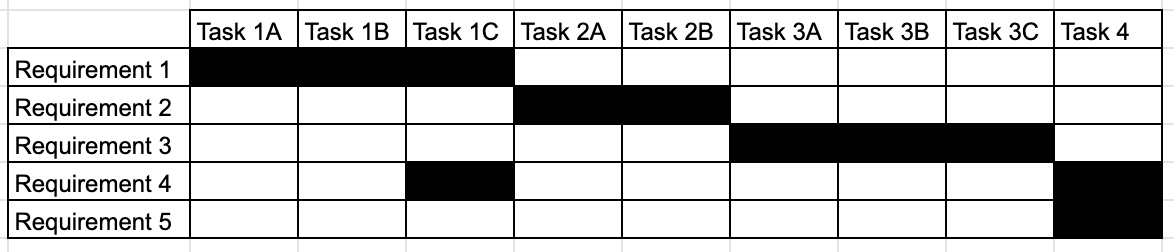
\includegraphics[width=0.9\textwidth]{Task_Matrix_01.png}
\centering
\end{figure}

In scientific research---I've seen it in the context of space missions or large instrumentation proposals---the RTM is sometimes reframed as the ``Science Traceability Matrix'' (STM). In this case, requirements are defined in relation to a set of scientific questions. For instance, if a scientific question is ``We want to assess the distribution of rocks with diameters between 0.2 and 1 meters.'' one of the requirements might be ``The system must be able to resolve rocks with diameters of 0.2 meters.'' or just ``Resolve 0.2 meter rocks.''\footnote{Here is a slide deck describing STMs by Sabrina Feldman at the NASA PI Launchpad Workshop (Nov. 9, 2019): \url{https://science.nasa.gov/science-pink/s3fs-public/atoms/files/Launchpad_Session3_STM_18Nov2019_smf_final.pdf}} Rather than mapping requirements to tasks, sometimes tests are used as a proxy; each test must verify the fulfillment of at least one requirement. This might be more accurately called a Test Traceability Matrix.

It is not mandatory that you create any traceability matrix, but it can be a useful additional way to visualize the relationship between requirements and other aspects of your project. It tends to be more useful for larger projects with complex relationships between objectives and execution. You can keep the traceability matrix in your records for your own project planning or management purposes. They also look good in proposals.

\newpage
\addcontentsline{toc}{section}{step six: project estimation}
\section*{step six: project estimation}

\epigraph{Estimates don't need to be perfectly accurate as much as they need to be useful.}{DtBA}

\subsection*{Make initial estimates of work effort by task}

Now you can finally begin to estimate! Start by going down the list of tasks in your Work Breakdown Structure and deciding how long you think each one will take to do in engaged work hours. Another way to think of this is ``billable hours.'' Don't include things like how long it takes to run a big simulation that doesn't require your active attention, nor time spent waiting for inputs or feedback from other people. Your assessment can be based on relevant past experience, if you have any. It can be based on a sense of how complex or difficult the task might be. It can even be based on raw gut feeling, if that's all you have. (Repeated or recurring tasks are a special case. See Appendix A of this document for more discussion.)

If they are available, the people who will do the task should be the ones making these judgments. If two or more people will be involved, they should discuss and arrive at a consensus. The consensus should not be a compromise. If one person thinks a task will take two hours and another person thinks that task will take ten hours, and neither of them can be convinced that their judgment is clearly wrong, take the larger estimate: go with ten hours. The reason is that there is a limit to how quickly a task can be completed, but no limit to how long it might take, so the truth is more likely to lie in the direction of pessimism.

If you don't know who will be doing the work, then I suggest that you imagine that whoever ends up doing the work will be mediocre at it. Perhaps assume that they are half as good as you, or only as good as your least competent colleague. If the person is going to be some future grad student or postdoc, perhaps imagine yourself early in your career and think about how long the task would have taken you then. Do this even if you expect to hire extraordinary people for the roles. We all hope to only hire and work with the best people, but we don't have total control over that, and even the best people sometimes perform poorly for a bunch of perfectly valid reasons. Similarly, you should not assume that you or your staff will be unusually productive; you will almost certainly tend to be about as productive as you've always been.

Don't fall into the habit of assigning some \emph{de minimis} amount to tasks that seem ``easy.'' Many things that you think are easy are not, once you get into them. And not everything that is easy is quick! As a general guide, your initial estimates should be at least a few hours for most tasks. If you are coming up with initial estimates for a lot of things that are less than four hours, then you are probably being too optimistic about how long things take or you have broken tasks down too far. DtBA also suggests that any task estimated at more than about 2 days of effort should probably be broken down more finely; my advice is to verify whether it makes sense to break any long tasks down more while recognizing that, in research contexts, it often does not.\footnote{Some examples that come to mind: (1) Writing a paper. (2) Attending a conference. (3) Periods of time devoted to purely exploratory research effort, e.g. literature review or ``playing with the data.'' (4) Long-running data QA or process babysitting.}

Be aware that people sometimes---consciously or unconsciously---fudge their own estimates downwards because they imagine that someone more experienced or more senior or smarter or better could do the work faster. So maybe they feel like they should be able to do it faster or should at least not get paid for doing it slower. You should fight that impulse. How long it might take someone else to do the work is irrelevant. It is probably true that someone else could do it faster, but unless that person is available and willing to do it, then it makes no difference.


\subsection*{rate your confidence of initial estimates}
\label{scrivauto:36}

Next, look at each estimate you just made and assign it a confidence rating between 1.2 and 4. Use 1.2 for tasks that are very similar or identical to something you've done before, and for which you have little question about how to proceed successfully. Assign a 4 to tasks that are entirely novel. Don't bother using more precise fractions. Just use 1.2, 2, 3, and 4. The extra ``precision'' won't gain you anything.

\subsubsection*{confidence ratings}
\label{scrivauto:37}

% make this a table instead?
\begin{itemize}[wide, labelwidth=!, labelindent=0pt, font=\bfseries]
\item[1.2]---You can apply this value to a task if you have deep domain expertise and have done something very similar to that task in the past. For example, if you have pre-existing code that you think that you can reuse with only very minor modifications---meaning less than 2 hours of work---then this is a good uncertainty factor. This is also a good scale factor for medium-effort tasks (cumulative days to weeks) which must be performed but which can most likely be cut short or rushed without propagating serious project risks. Things like ``literature review'' or ``hands-on testing with beta users'' sometimes fall into this category.
Note that the number is not exactly 1. This is because people underestimate how long things take, even things that they have done before.\footnote{
Unless they have carefully tracked and logged the effort, repeatedly. Many businesses do this, but very few individuals.}
It is therefore safer to assume that everything will take longer than you think. This is also a good uncertainty factor for tasks that have a known, fixed duration, like perhaps a 2-day (16-hour) design review, or a 1-week (40-hour) conference. Why don't tasks with known fixed durations merit a scale factor of exactly 1? Because you should arrive a few minutes early to every meeting and meetings rarely end on time! Or you might be asked to ``stay after'' for some followup discussion. And even ``fixed duration'' tasks have switching costs---the overhead associated with initiating and concluding a task---which you should account for.

\item[2]---You can apply this value to a task if you have deep general domain expertise in that task, but have not done very similar things in the past. More broadly, you can use this value for tasks you otherwise regard as ``easy.'' (Yes, your estimate of how long it will take you to do an easy thing is probably wrong by a factor of two. It's probably wrong by at least a factor of two!) When I am scoping categories of work that I regard as ``engineering tasks'' (e.g. implementing feature sets that do not require novel algorithm development or other ``research'' in order to figure out how to do them at all), this is the most common scale factor that I use. When I need to quickly estimate small-scale projects (hours to days of effort, with only a handful of requirements) that are in my general domains of expertise, I will often just multiply my initial estimate by 2.\footnote{If we didn't have a justifiable system behind the decision to multiply by two, we would just be ``padding'' the estimate, which is a word often slung with contempt and derision, especially by people who think that the point of an estimate is to be accurate instead of useful, or who have trained their their engineers to lie to them. When the total project size is small, then the costs associated with spending several more hours making the estimate ``better''---not more accurate!---almost certainly gives a terrible marginal return on investment.}

\item[3]---Apply this value to tasks in the space between 2 and 4. You might have some domain expertise and some idea of how to go about completing them, but not total confidence in either. Alternatively, you might have deep domain experience but no clear idea about how to complete the task. Perhaps there are undefinable confounders in the requirements or aspects of the work that won't be clear until you start; these may push a ``2'' task into a ``3.'' Anything that is ``more than 2'' and ``less than 4'' gets a factor of 3.

\item[4]---Use an uncertainty factor of 4 if you have a strong sense that a task is possible to achieve, but almost no concrete understanding of how to go about achieving  it. Developing high-performance physical simulations will often carry this kind of uncertainty, as designing and optimizing algorithms often composes the ``research problem'' itself. This factor can also be appropriate for a task that simply seems very hard to you. Remember that it's irrelevant that it might seem easy to someone else, unless you can hire that person.
\end{itemize}

It is worth mentioning that this scale is not arbitrary. It's not a ``fudge factor'' or a ``pad,'' and you should bristle at anybody who tells you otherwise. TPMG notes that Boehm et al. (1995) examined ``the range of possible errors in the estimates of cost at various points in a product's development'' and found that ``[W]hen the concept of the software is being developed [{\ldots}], the estimate can be low or high by a factor of 4 (that is, 4x to 0.25x).'' Given, as we've previously discussed, that the nature of research funding requires that our estimate be sufficient, we should not entertain at all the possibility that our initial estimate is too high, and can therefore eliminate all of the factors less than one. (That is to say---in case this wasn't clear---that you should not ever scale any of your initial estimates \emph{down}.) DtBA uses this same range at the stage of ``initial concept'' (citing Boehm et al. 2000), and further notes that this is ``the error in estimates created by skilled estimators. It's easily possible to do worse. It isn't possible to be more accurate; it's only possible to be more lucky.'' Many sources note that the distribution of the wrongness of estimates tends towards a Pareto distribution (as so many things do), and this method incorporates that aspect as well.\footnote{
We're about to do a pairwise multiplication of two lists of random-ish numbers. If you take a list of random numbers distributed evenly across some interval and multiply it pairwise by another list of random numbers distributed evenly across some interval, the resulting values approximate a power-law distribution.}

As before, the people who will actually be doing the work should be making these assessments.\footnote{
DtBA suggests that you should have ``one person create the `how much' part of the estimate and a different person create the `how uncertain' part of the estimate.'' This mitigates against the first part contaminating the second part with your own biases. It was also written for a context in which (most of the time) the people who will actually do the work are not deeply involved in the estimation process. You also probably don't have enough people to silo some of them for half the effort. Rather, I trust that you will do your best to forget your initial estimates when defining your uncertainty factors.}
If those people aren't available, then you should probably assign \emph{at least} a factor of 2 to all of their task estimates. If you would give it a 4 if you were going to do it yourself and you aren't confident that whoever does the work will have special relevant skills, definitely consider giving it a 4.

If you are doing the estimation with a team, at some point, you're going to have two people who will share a task get stuck with scale factors that are off by one, unable to agree to move their uncertainty up or down. Often someone will propose that they just split the difference, use a decimal fraction, and move on. I believe that compromise of this type rarely actually gets you closer to the ``truth.'' But if you want to split the difference, or, more importantly, if it allows an otherwise stalled estimation process to move forward, then go ahead and use half-points as well. (I really believe that seeking a level of precision beyond that is tilting at windmills.) However, if two people doing the estimation exercise disagree on the scale factor by more than one point, you probably want to force the discussion to continue until they come into better alignment---or just use the higher value.\footnote{
And if one person assigns a 4 to a task---meaning that they don't have a clear idea about how they'd go about the work---and someone else assigns any lower number, then it should be resolvable to at least a 3 on the spot by having the second person explain it to the first one.}

\subsection*{generate your estimate(s)}
\label{scrivauto:38}

You now have initial time estimates for all tasks and uncertainty factors associated with each of those. What you do with them at this point depends on the goals of your estimation process.

\subsubsection*{what is the best case scenario?}
\label{scrivauto:39}

The sum of your initial estimates for all tasks (ignoring scale factors) is the estimate for how long the project would take if everything went exactly according to your expectations. We'll take this to be the best case scenario. It is the minimum required work effort necessary to do the project. As we discussed earlier, for most research software projects, the work effort will be the main driver of the total project cost. This means that you can take this best-case estimate, multiply it by the fully loaded salary costs of your team members, and get an estimate of the total amount of money required to do the project. If this is more money than you have or can ask for, then the project is probably not feasible. You should go back to the beginning and try to come up with a more efficiently-implementable solution, be less ambitious about scope, or maybe give up the idea altogether.

\subsubsection*{how much money should I ask for?}
\label{scrivauto:40}

The sum of your initial estimates multiplied pairwise by their corresponding confidence factors is the Project Estimate. This is the amount of work effort that provides a good chance of project success, as long as nothing major was left out of the scoping and estimation process. Although it can feel sort of ethereal, this number is not a ``guess'' and it is not ``padded.'' You used an approach derived from well-tested best practices for software project estimation. Your number is reasonable and it should be sufficient. These are typical merit criteria for research proposals: that the requested resources are both ``reasonable'' and ``sufficient.'' So this is the number that you use as the basis of your proposal budget.

\subsubsection*{how long is the project most likely to take?}
\label{scrivauto:41}

This is the question that most people think that they want to answer when they request an estimate. The estimate methodology just described does not yield a straightforward way to make this assessment. Even if it did, it would be so misleading as to be useless. Estimation methodologies intended to produce expectation values have a lot more inputs and also produce confidence intervals, which are often quite large ($>$30-50\%). But if you must have this for your own private purposes, I suggest you place it at about 75\% of the range of the numbers in A and B. So if your Best Case is 100 hours and your Project Estimate is 300 hours, you can place your expectation value around 250 hours. But, first, don't trust this number at all, because it has almost no basis in reality and is probably super wrong. And, second, you should probably never tell anybody this number, especially if you work for them or they control your funding, because they are as likely as not to take this as your actual estimate, incorrectly write off the Project Estimate as having been ``padded,'' and cut your support to 75\% of what you need to be confident of success. In fact, forget that I said anything. Go wash your hands.

\hfill
\begin{mdframed}[everyline=true]
\textbf{Summary instructions for a project estimate.} Make an initial time estimate for each project task in hours of effort or equivalent. For each estimate, assign an ``uncertainty factor'' of 1.2, 2, 3, or 4, where 1.2 is assigned to tasks that are very well aligned to your prior experience and 4 is assigned to tasks that lie outside of your prior experience or expertise. The sum of estimates of each project task is the lower bound, or the minimum amount of effort required for the project if nothing goes wrong. The sum of pairwise products of task estimates and uncertainty factors is your Project Estimate, or the amount of effort that is likely to be reasonable and sufficient.
\end{mdframed}

\newpage
\addcontentsline{toc}{section}{apologia}
\chapter*{apologia}
\label{scrivauto:43}

\section*{estimates are wrong}
\label{scrivauto:44}

Keep in mind that all estimates are wrong. When you make an estimate---especially at the outset of a project, or in the proposal phase---you are trying to figure out what it will take to solve some big problem or set of problems over months or years at the time when you have the least information about possible solutions and difficulties that you might encounter. This is almost futile! Even people who do it professionally and can draw upon mountains of data, including historical performance on similar projects, are not very good at it. Academics managing software projects incidental to their research should not expect to do better.

Also, estimates are not predictions. They're not supposed to be predictions. Even if they were, they could at best provide accuracy without precision. (e.g. ``It will probably take 1000 hours and definitely won't take less than 1 hour or more than 10 years.'') You should judge your estimates by how useful they are, not how accurate they are.\footnote{This is a point that SEWG hammers on a lot, and I agree completely.} In the case we're talking about---smallish software projects as part of grant-funded research---an estimate is useful if it helps you request sufficient resources to achieve project success without being unreasonable.


\section*{an estimate is not a negotiation}
\label{scrivauto:45}

At some point you will encounter someone---maybe yourself---who wants to treat your estimate as the opening salvo of a negotiation. You might go through the whole process outlined above and find that you need 500 hours of work, but can only request support for 350 hours of work. Or when you tell your boss 500 hours, he might ask if you can do it in 250 instead. In cases like this, you may find yourself thinking that you can just work harder and make up the difference somehow. You might think it's better to close the deal or make your advisor happy and that you'll figure it out later.\footnote{
A number of managers—especially in STEM fields—seem to have learned their management style from a particular science fiction universe that I have previously referenced for modeling particularly dysfunctional management workflows.}

Do not do this! Never negotiate an estimate. You'll be setting yourself and your project up for failure. Instead, in these situations, negotiate the scope of the project and then re-estimate. For the project to take less time, it must do less. Alternatively, you can try to negotiate the available resources. If the project is going to do more, then it needs more time. But the estimate itself is not open for negotiation.

As an alternative to rescoping, you can try to brainstorm new approaches, technical solutions, or designs which might propagate to lower estimates. But if broader changes to your approach are needed, then you should return to the ConOps phase and re-estimate the project as a whole. This is likely to feel like distracting non-work at a time when you might be under increased pressure to produce. The temptation to not reassess the project will be strong. But if there really is a large mismatch between your estimated resource needs and available resources, the project is probably at very high risk of failure, and that can only possibly be mitigated by a new approach. If you are lost in the woods, often the best thing to do is sit down and carefully re-assess the situation.

\section*{the estimate is not the plan}
\label{scrivauto:46}

Specifically, the amount of budgeted work effort that we've just calculated is not the same as the amount of calendar time that it will take to complete the project from start to finish. If you need 4000 hours or 2 FTE for the project, that does not mean that one person can or should finish the project in two years of working flat out. There are many reasons for this. One is that a lot of project tasks will only be possible to complete in sequence, because outputs of one task are inputs to another. Another is that you might need to wait for inputs almost entirely external to your project---maybe call them ``bottlenecks''---like responses from colleagues or specific data to be collected by space telescopes or on field work. The upshot is that the work effort that we've calculated---or ``billable time,'' as I think of it---is almost always much smaller than the calendar time from project start to finish. We will discuss generating a plan from the estimate in the next section.

\newpage
\addcontentsline{toc}{chapter}{project planning in brief}
\chapter*{project planning in brief}

A project plan is often represented in the form of a Gantt chart, which is a table, bar graph, or timeline with time on the horizontal axis and tasks on the vertical axis, delineating in which window of time each task will occur. Given that our estimation method only provides hours worked, it is a very good idea to generate a Gantt chart to establish whether the project can fit within whatever total amount of calendar time is available for the task, and what amount of continuous or sometimes instantaneous effort that will require. It is also a very good idea to include a Gantt chart in your project proposals. In Appendix B, I have included two examples of Gantt charts for real projects that I put into my own proposals; you should probably refer to these while I attempt to describe how to create one in the next few paragraphs. There are, of course, a number of software packages to aid in creating Gantt charts, including some open source options that---as far as I can tell---are perfectly functional. But my preference at the scale of a research effort is to just use a spreadsheet.\footnote{
This is partly just because I haven't been motivated to take the time to learn a new tool. I suspect that the amount of time it takes me to generate or update a Gantt chart could be cut to at least a quarter if I used the ``right'' software, and there will come a point—probably soon—when it's overwhelmingly worth it for me to take the time to learn. Spreadsheets have other benefits, though, like that they are easy to distribute, most of my collaborators are quite comfortable using them, and I have deep control over format and data representation.}
	
Along the top row of the spreadsheet, make date ranges at 1- or 2-week, 1-month, or 3-month intervals, depending on what seems most appropriate to the project. If there is a fixed or notionally fixed time frame for the project, e.g. for a 3-year research effort, then cap the intervals at that duration; otherwise intervals can be added or removed as needed. For multi-year efforts, you may also want to delineate project years (as opposed to fiscal or calendar years) because this is typically how grant programs want budgets and work effort to be reported, and it is very convenient if your Gantt can quickly be cross-referenced to your budget. Along the left side of the spreadsheet, list every task from your previously created work breakdown structure. In the next column, as a reference, put the amount of effort in hours or FTE (your choice) that you have estimated for that task.\footnote{This will be the initial estimate for the task multiplied by its scale factor. Astute readers may object that the utility of estimates of individual tasks is far less than the utility of the sum of estimates of these tasks which comprises the total project estimate. This is because we count on the cumulative wrongness of the task-level estimates to smooth out at the project level. So for project planning purposes, maybe think of the task-level estimates instead as something like ``fungible resource allocations.'' Once the project is underway, some tasks will take less time than estimated, and that will allow you to put more resources into tasks that inevitably take more. The annoyingly astute readers will also object that not all personnel time is fungible, especially if tasks require specific expertise that only one person on the project has. That's also true, but I don't know what to tell you except that I'm sure you're pretty clever and you'll probably figure something out. Attaching fungible vs. non-fungible personnel to tasks is a feature offered by real project management software, if it's a feature that you really want.}

Some tasks may be fixed in time. For example, if you are planning to present at specific conferences, those dates are probably known, or you at least know which month or quarter they will occur in. You might also have field work that must happen in a particular season of a particular year of the project. Some deliverables may also have specific due dates within the project, as we've already discussed. Fill in the cells corresponding to these tasks and time intervals with the associated estimated task effort. While other tasks can be juggled around in time and duration, these are fixed anchor points.
	

Now, using the WBS as your guide, establish which tasks and subtasks are inputs to others and which can be done in parallel. The relationship between these tasks in time should be obvious: the dependencies of a task must be completed or nearly completed before the task can begin. If it's not obvious---or maybe even if it seems obvious---it is probably a good idea to discuss these dependency relationships with the team before locking them in. It can be helpful to list out all of the tasks and then draw arrows between them, indicating inputs and outputs. (Indeed, some Gantt charts even incorporate arrows.)

Fill in cells for these tasks with their associated time estimates in a temporal arrangement that respects the directional dependencies; that is, the dependencies for a task should occur before the task. For now, just fill in one cell per task. You should have something that looks like the following, where Task 1A is an input to Task 1B and so forth.

\begin{figure}[h]
\centering
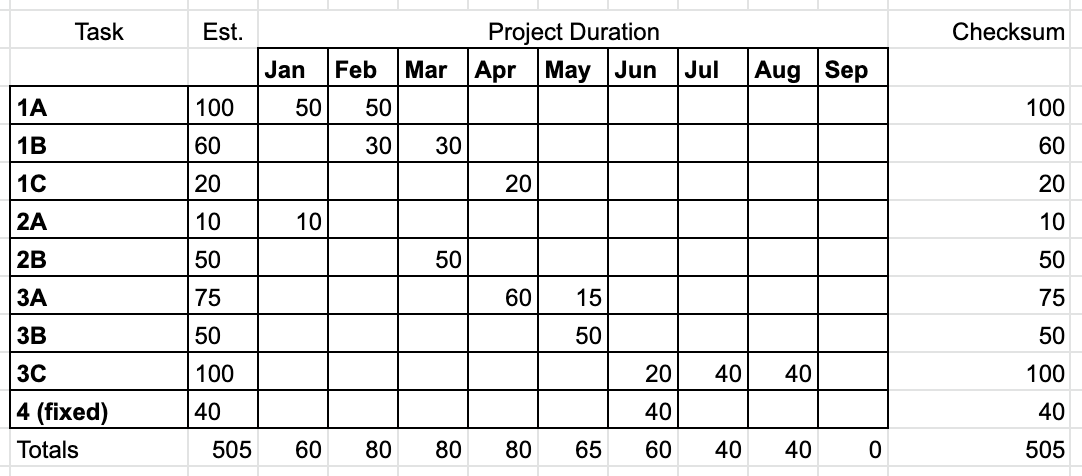
\includegraphics[width=0.8\textwidth]{Plan_01.png}
\centering
\end{figure}
\break
Your task might all fit into the chart like this, emanating as they do from the project start. If your tasks already run off the right side of the chart, i.e. you run out of time for the project before everything is completed, then you might have a problem! You might also just need to use a shorter time step.
	
Make sure that the total work effort on each sub-project, task, and the project as a whole adds up to the numbers given by the project estimate; you can do this by summing over rows in the spreadsheet to generate a ``task total'' column on the right side and also summing along columns to generate a ``project total'' row along the bottom. The ``task total'' should be equal to the task estimate in the second column, and the ``project total'' should be equal to the total project estimate.

You should verify that the total effort in any given time interval does not exceed the total possible amount of effort that your project team can produce in that time period; for example, two people cannot work more than 80 hours in a week or 1040 hours in a quarter. Let us assume in the notional project above that what we have available for this project is one person working at half-time. This means that they have 80 hours per month to devote to the project. Nearly every month of the project currently calls for more effort than this! So we need to spread the effort out over time more. We do this by expanding the duration of each task and also shifting the tasks in time so that the total effort in each time interval does not exceed what is possible. It's a bit of a puzzle for which there are multiple plausible answers, and sometimes none. Here's an attempt to do that for the example above:

\begin{figure}[h]
\centering
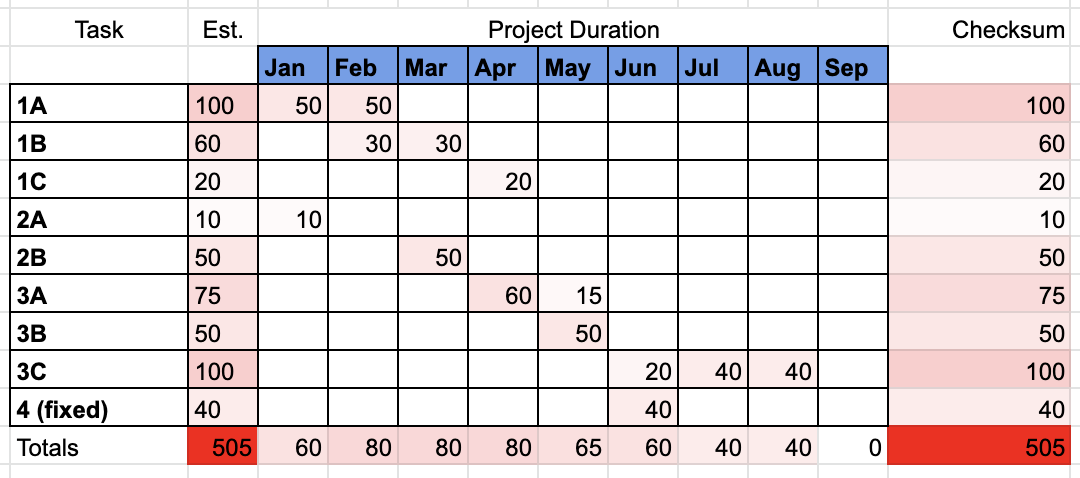
\includegraphics[width=0.8\textwidth]{Plan_02.png}
\centering
\end{figure}

I like to use the ``conditional formatting'' feature of the spreadsheet software to color each cell of the chart from white to an increasingly full red based on what fraction of the total time to the project is allocated to that interval of time (or cell in the spreadsheet). I also color-code the ``total'' row at the bottom of the Gantt chart in the same way, where the sum along each time interval is weighted according to the fraction of the total estimated FTE that it contributes. What I am looking out for with this is any unusual spikes in effort required at any point during the project. It is better to not have those, and to try to smooth them out if possible, because there will often be logistical and real costs to ramping effort up and down quickly; steady and consistent is generally better (although there are sometimes good reasons for periods of sprint), so most of your cells along the bottom row should end up sort of pale pink-ish.\footnote{
The linear color ramp from white to red works well for me, but there's nothing special about it. Code your chart however works for you. Or read something by Edward Tufte and make an informed decision.}

Obviously you can fiddle with this endlessly, and you should fiddle with it some, and debate the merits for various plans and whether there are aspects of the project or timeline that you are forgetting and need to factor in, etc. Much as with project estimation, this kind of project planning comprises an entire field of study and domain of expertise, of which the prior few paragraphs barely even qualifies as a gloss. But I think it's mandatory that a proposal includes a Gantt chart, and this should be enough to get you started. If you have a complicated project or life or property is on the line, work with an experienced professional! Also as with estimates, you should revisit your project plan regularly once the project is underway and revise it completely if the project scope, timeline, or estimate changes. Reality will diverge from your plan; be prepared to adjust and adapt when that happens.

\newpage
\addcontentsline{toc}{chapter}{putting it into the proposal}
\chapter*{putting it into the proposal}
\label{scrivauto:49}

\label{scrivauto:50}

\epigraph{If you want to keep something secret, \\write it down!}{Dai Vernon}%\footnote{Dai Vernon aka The Professor was among the greatest performers, teachers, and philosophers of theatrical magic of the 20th century and certainly one of the most important magicians to ever live. I might not qualify it at all except that he shared part of the century with Houdini, who he famously fooled with a card trick. He was referring in this quote---which I've been told he often repeated with slight variations---to writing magic secrets in books, which many people are astonishingly reluctant to read. (When I do magic tricks for people, and they ask me how they are done, I sometimes offer them access to my library where the explanations for that and more can be found. Only one person has ever taken me up on the offer.) It's my experience that the sentiment applies equally well to software documentation and journal articles! Vernon also used to say, "Magicians stop thinking too soon." We could substitute many nouns.} \hfill \break

\label{scrivauto:51}

All of the hard work that you've done on project scoping, estimation, and planning will amount to very little if you cannot get the resources necessary to carry out the project. It will be much easier to convince people to trust your estimate and plan if they understand the method you used to generate them, and that this method has a legitimate basis and is not merely ``a guess.'' If you only need the assent of your boss or PI, then you will probably have the luxury of explaining the process to them, answering their questions, addressing their concerns, giving them a copy of this document, etc. But if you're writing a proposal, your job is harder. You must make your appeal to a handful of anonymous people, probably strangers, who are unlikely to have backgrounds in project management or systems engineering, who might not have much background in software development, and who are required to judge the merit of your request based on nothing more than the text and graphics that you've managed to cram into your page allotment. It has taken me nearly 20,000 words and 50 pages to explain the process, so what hope do you have?

Some. Because the reviewers do not need to fully understand the methodology. They only need to believe that a methodology was used and that it is not bullshit. Here is an example of actual language that I put in one of my proposals, which I hereby grant you permission to use as a model for your own.\footnote{I only ask that you cite this document. Information on how appears at the end.}

\begin{displayquote}
To assess project feasibility and requirements, we used a project estimation approach that we have adapted from commercial practice and modified to be more appropriate for the high-uncertainty environment of cutting-edge research. We broke the project down into major tasks and then subtasks as needed to reach a granularity where every well-defined unit of the project had a scope that we could conceive of accomplishing. We then estimated the level of effort (LoE) required for each subtask. Initial estimates were based on our prior experience doing similar work [when possible]. We then assigned an `uncertainty' scale factor of greater than 1 to each estimate as a rough measure of how confident we were in our initial estimate. For example, a situation in which we planned to identically recreate work that we'd done previously would be considered very accurate and assigned a scale factor of one. A situation in which our initial estimate was only a guess, perhaps because it was in a domain with which we had little experience, might be assigned an uncertainty factor of 3 or more. Given our extensive prior experience with projects of this type, none of our scale factors were greater than 2. The PI and Co-I iterated on and agreed upon LoE and scale factors before proceeding. The sum of the initial estimates forms the lower bound on the estimate: the LoE required in the case where the project proceeds exactly according to our expectations. The sum of initial estimates multiplied by their uncertainty factors forms the upper bound of our estimate: the LoE necessary to guarantee project success. We ran the estimation exercise twice. In the second round, some of the subtasks were refactored based on discussions about methodology and technical approach. We did not reference the first estimate during the second, but both returned similar results (within 0.1 FTE\footnote{I consider 0.1 FTE or anything $<$10\% to be a rounding error, given all of the possible sources of uncertainty leading into this number. You are allowed to round your bottom-line estimate up to the nearest 0.1 FTE; more precision than that is an illusion. The agreement after re-estimation was an accident. We weren't trying to validate our estimate by doing it again. Rather, after the first project scoping and estimation exercise, we thought of some alternative technical approaches to elements of the project that we suspected might be more efficient. It turned out that there was almost no difference, at least as far as the estimate could tell us.
}): 1.5 FTE is the minimum required effort for this project, and 2.5 FTE is necessary to guarantee project success. We are requesting support for 2.66 FTE, which includes 0.3 FTE of a TBD undergraduate intern from a nearby university who we expect to work at lower efficiency than the professional-level programmers (of approximately our own abilities) assumed during this estimation exercise. We are confident, therefore, that the requested level of support is both reasonable and sufficient to complete the proposed project.
\end{displayquote}
\vfill
This concludes the whirlwind overview of research software project estimation. Know that it is an art as much as it is a technology, and your outcomes will improve with practice and experience. \emph{Any} amount of effort put into project scoping, estimation, and planning puts you far ahead of most and will result in better research software. Good luck!
\hfill \break \hfill \break \hfill \break

\addcontentsline{toc}{chapter}{bonafides of the author}
\chapter*{bonafides of the author}
\label{scrivauto:52}

\label{scrivauto:53}

\epigraph{So fare thee well, \\poor devil of a Sub-Sub [{\dots}]}{Moby-Dick; or, The Whale} \hfill \break

\label{scrivauto:54}

This whole thing is written in the first person, so I should probably introduce myself. You might also want a basis for deciding when to listen to me and when to ignore me. My name is Chase Million. I own a research, software, and consulting company called Million Concepts. I have nearly 20 years of experience writing software to support scientific research. This started as an undergraduate at Cornell University ca. 2003 working on the Pancam instrument team of the Mars Exploration Rovers, where I contributed to calibration and data analysis software tools (some of which are still in use today). My first job out of college was at Caltech, where I inherited the image processing pipeline for the Galaxy Evolution Explorer (GALEX), an all-sky ultraviolet survey telescope in low-Earth orbit.

I started Million Concepts in 2011 to try to improve my own practice of research software engineering in ways that I thought would be impossible---or at least much more difficult---from within a university or existing institution.\footnote{This is now a defined term. “Research Software Engineer” is a specific job designation, with an increasingly clear career progression, and (likely soon) a formalized training regime. There are even affinity / advocacy groups for this, such as the United States Research Software Engineer Association (https://us-rse.org). Like “Data Scientist,” this is not a term that existed when I was starting. And I admit to being a little bit of a hipster / curmudgeon about the fact that I was both a ``research software engineer'' and a ``data scientist'' before any of it was cool.
} Chief among these was that I thought that the existence of a contract between myself and the project PI would force us to have a shared understanding of scope and deliverables at the outset. This contract would mean that I would not waste my time making unwanted tools, and it would also provide me some recourse if the PI changed the project parameters drastically. If you've ever done any software development on contract, you are probably shaking your head or laughing at the previous sentence; my belief was naive and wrong! Nonetheless, in dealing with the fallout of my naivety---and the day-to-day realities of running a business---I was forced to learn about project scoping, estimation, budgeting, statements of work, and all of the other artifacts and processes around software project management and contracting that minimize headaches and maximize successes.

Much of our work at Million Concepts involves developing software in support of research in planetary science and astronomy. This includes doing data analysis, writing and maintaining calibration pipelines and analysis software, and preparing data for archiving or publication. At the time of writing, we are supporting the ongoing Mars 2020 and Mars Science Laboratory missions, analyzing Lunar observations by Arecibo Observatory and the Chang'E orbiters, improving the calibration and accessibility of the GALEX data, searching for rare signals in stellar flares with data from the TESS and Swift space telescopes, writing a software library that will support ~2 petabytes of observational data of planets held by NASA's Planetary Data System, and helping to develop the next generation of cloud-enabled access and analysis tools for digital astronomical imagery. These projects invoke a long list of popular keywords from software development and technology startups over the past decade: big data, high performance computing, cloud computing, user experience design, data science, machine learning, and so on. Such is the exciting, multidisciplinary nature of research software engineering!

I have no formal training in software development or project management and only a little bit in engineering. I also do not have any advanced degrees. While I have certainly had mentors, most of what I know about software development and software project management has been learned from reading and experience. I'm starting to think some what I've learned is correct. I hope that you have found some of it useful.

\newpage
\addcontentsline{toc}{chapter}{recommended reading}
\chapter*{recommended reading}
\label{scrivauto:55}

\label{scrivauto:56}
\begin{itemize}[wide, labelwidth=!, labelindent=0pt]
\item ``Software Estimation: Demystifying the Black Art'' (DtBA) by S. McConnell
\item ``Software Estimation Without Guessing: Effective Planning in an Imperfect World'' (SEWG) by G. Dinwiddle
\item ``The Project Manager's Guide to Software Engineering's Best Practices'' (TPMG) by M. J. Christensen and R. H. Thayer
\item IEEE Std 830-1998 ``IEEE Recommended Practice for Software Requirements Specifications''
\item ``The Missing README: a guide for the new software engineer'' by C. Riccomini and D. Ryaboy
\item ``The Startup Owner's Manual: The Step-By-Step Guide for Building a Great Company'' by S. Blank and B. Dorf
\item ``Clean Code: A Handbook of Agile Software Craftsmanship'' by R. C. Martin 
\item ``Working Effectively with Legacy Code'' by M. Feathers
\item ``Visual Explanations'' (and all other books) by E. Tufte
\item ``Science in Action: How to Follow Scientists and Engineers Through Society'' by B. Latour
\item ``The Golem: What You Should Know About Science'' by H. M. Collins and T. Pinch
\item ``Thinking, Fast and Slow'' by D. Kahneman
\item ``Moby-Dick; or, The Whale'' by H. Melville
\item ``Illuminatus!'' by R. Shea and R. A. Wilson
\end{itemize}

\addcontentsline{toc}{chapter}{acknowledgements and license}
\chapter*{acknowledgements and license}
This work was supported by the Better Scientific Software Fellowship, part of the Exascale Computing Project (17-SC-20-SC), a collaborative effort of the U.S. Department of Energy Office of Science and the National Nuclear Security Administration. The text benefited from feedback and copy editing by Michael St. Clair (Million Concepts), Dmitry Savransky (Cornell University), and David Mayer (USGS). Any errors or omissions are the author's fault.
\hfill \break \hfill \break
\href{http://creativecommons.org/licenses/by-nc-sa/4.0/}{This work is licensed under a Creative Commons Attribution-NonCommercial-ShareAlike 4.0 International License.} Please cite
\hfill \break \hfill \break
\texttt{Million, C. (2022, May 25) A practical guide to research \\software project estimation (Version 1.0) Zenodo. [DOI TBD]}

\addcontentsline{toc}{chapter}{appendix a: recurring tasks}
\chapter*{appendix a: recurring tasks}

If you have a task that repeats, you can estimate the task once and use a sum across all repetitions.\footnote{DtBA refers to this as estimation by ``counting.''} If you expect the repeating task to be about the same amount of effort every time, then you can just make one estimate and multiply it by the number of repetitions. Sometimes a task repeats for the most part, but the details of each iteration could make them take variable amounts of time. In those cases, you might want to use some simple distribution for your estimates that is rooted somehow in your understanding of the problem / tasks. A commonly useful heuristic, for example, is to assume that the effort will fall along a power law distribution. Many things \emph{do} tend to fall along power law distributions, after all.\footnote{Like the accuracy of estimates.} You might also have heard of this as the ``80/20'' rule in which 80\% of the thing takes 20\% of the resources, or vice versa. (Statisticians call it ``the Pareto distribution.'') So you could say, ``This task will recur 100 times. I think that most of those will take 8 hours. Some will take more.'' How many will take 8 hours? Maybe assume that it's 80\% of them. And how long will the other 20\% take? Well one quarter as many will take four times as long, so 32 hours. (You could extend this to three discrete tiers, but more than that is probably overkill. You could calculate it as a continuous variable, but I think that's super-overkill.)

Other distributions that you might consider are:
\begin{itemize}[wide, labelwidth=!, labelindent=0pt, font=\bfseries]
\item[Gaussian:] Where the majority of the repetitions ($\approx{70}\%$) will take an average amount of time, and ($\approx{15}\%$) will take a small amount of time, and ($\approx{15}\%$) will take perhaps half as long and ($\approx{15}\%$) will take twice as long.
\item[Decaying:] If you expect to get more efficient or faster at the task over time, or if there is an economy of scale, then you might model that with a downward trend. So that the first 20\% takes N hours and the second 20\% takes N/2 hours, etc., at whatever rate of decay you think is reasonable.
\item[Increasing:] If each iteration will become more complex and therefore take more time. I can imagine this happening, for example, if this is a ``data validation'' or ``data cleaning'' task, and the total volume or sources of data is expected to be larger each time. Perhaps you are writing a calibration pipeline for a project that is actively collecting data, and you plan to completely reprocess the data annually with the latest version of the pipeline. While the software runtime itself should not necessarily be factored into your estimate (of ``billable hours''), the mere fact of increasing data volume over time most likely means that bookkeeping, process babysitting, validation, and data delivery will take longer each time.
\item[Bi-modal or multi-modal:] Where known fractions will take specifically different amounts of time (in two or more bins). This particularly makes sense in a case where you have a task that repeats but some of those repetitions will have extra steps or complexities that themselves can be estimated, and you know the approximate fractions ahead of time. If you're not using continuous distributions anyway---which you shouldn't---then this is really just the general case option. (You could make it look like any distribution you wanted.)
\end{itemize}

\section*{example of estimating a recurring task}

At the time of writing, I'm leading a project to develop a software library---the Planetary Data Reader (pdr)---that will be capable of reading the ~2 petabytes of observational planetary science data held in the Planetary Data System.\footnote{https://github.com/millionconcepts/pdr} The PDS (and the affiliated International Planetary Data Alliance) is the central archive for data from planetary science missions---Apollo, Voyager, Mars rovers, orbiting spacecraft, etc.---, including all NASA missions and many international missions, dating back more than fifty years. In that time, standards and practices for archived data have shifted substantially, to say nothing of data formats and computer technology. And with so many different people preparing and submitting data to the archive over so long, the quality and adherence to standards are all over the place. The result is a vast trove of extraordinarily valuable data, of varying type, some of it low quality, and with documentation ranging from absent to superb. How could we estimate the task to support all of this data? This is what we put in the proposal:

\begin{displayquote}
The required level of effort for this project is clearly a function of the number of unique ``data product types'' archived in the PDS. However, that number is not available. Nobody has cataloged the data in that way, as far as we know---and we have asked many people. The number of separate instruments from which observational data has been archived, however, is a reasonable proxy. This can actually be calculated with some accuracy because ``INSTRUMENT\_NAME'' or some equivalent is a standard metadata label in every PDS data set we have ever seen. (Of course, there are PDS-archive data sets that are not the output of specific instruments, but these were relatively rare until recently, when moves toward scientific reproducibility have encouraged more scientists to archive the output of their R\&A projects, rather than only the data output from missions. More recently archived R\&A output should be subject to the strict requirements of [PDS version 4 standards] and therefore pose almost no issue as far as accessibility.) Per information provided to us by [PDS] staff following a request for a count of unique instruments archived in the PDS, we estimate that the number is ~600. We then also estimate that the ``difficulty'' of reading the data follows a Pareto distribution. This is a common heuristic in software project management, often called the ``80/20 Rule:'' 20\% of the project will take 80\% of the effort. Following this heuristic, we estimate that 80\% of data types will be relatively easy to provide read support for (~2 hours), 16\% of data types will require a moderate amount of additional effort (~2 days or 16 hours), and the remaining 4\% of data types will require a relatively large amount of effort (~2 weeks or 80 hours). The Pareto distribution is a good heuristic in many situations where precise information is not available, but also comports with our impression of the data and associated difficulties based on our prior experience working with planetary science data generally and prototype the Planetary Data Reader specifically. The result of the analysis is that ~2 FTE is required.
\end{displayquote}

There are two things to note here, because they seem to contradict things that I've said before. The first is that I said that I think it's a good guideline that every task takes at least four hours, and yet here I've claimed that 480 tasks will all take only two hours each. Repeated tasks are an exception to that rule. Imagine that the task that you are estimating is to stuff 5,000 envelopes with letters for a political campaign. While you can certainly imagine doing this task (and that your arms would get tired), you probably have no basis for knowing whether it will take 4 hours or 40 when stated like that. But if you estimate that each envelope takes 20 seconds to stuff, then you can multiply that by 5000 and say that it will take about 28 hours. Whereas it would be ridiculous to insist that it takes 4 hours to stuff each envelope.\footnote{ It's 2.3 years of stuffing envelopes, but only six a day.}

The second note is that I have not used ``confidence'' scale factors on the time estimates. The reason is that I think they don't matter very much for repeated tasks. By the time that you do the task for the second time, you are by definition doing something extremely similar to something you have done before, which would merit a confidence interval of 1.2.\footnote{For this reason, I often treat the first iteration of some repeated task as its own task for the purpose of estimation, often with a description related to designing and setting up the task. So if you are stuffing 5,000 envelopes, there would be one task in the WBS like “Design / implement approach to envelope stuffing.” and another task called “Stuff 4,999 envelopes.”
}
By the time that you have done something ten times, you are almost certainly more confident than that. At the same time, as a scale factor that translates to a 20\% increase in the time estimate. To my thinking, this is a small number compared to the inherent possible uncertainty or ``slop'' associated with picking the initial estimate or model. However, it would not be outrageous to add 20\% to recurring task estimates, and, in hindsight, I probably should have done that.

There are obviously a lot of ways that one might choose to do this calculation, and it would be possible to arrive at nearly any result. For the pdr estimate, I could have just said that each data set will take about 10 hours on average and gotten a result of ~3 FTE, or used 7.8 and gotten exactly 2 FTE. I might have modeled this as a decaying estimate, where the time required for each new data set drops as the team gains experience. Heeding my own advice to not sample the distribution too aggressively, I would probably pick just four steps of 80, 40, 20, and 10 hours. The calculation would be $600 \times 0.25 \times (80 + 40 + 20 + 10) = 18,240$ hours, or $10.8$ FTE. For the scale of research grants that we are mostly talking about, this would almost certainly be too expensive to be possible.\footnote{Somewhere around \$1.1--1.7M.} Note that a multi-modal or Gaussian approach might have also been plausible, and could have led to different answers. After discussion among the team, we thought that the Pareto distribution was in fact the best match for what we knew about the problem at that point.\footnote{About one year into the project, we still think that this distribution is more-or-less the right one.}

You will need to try to maintain a mental barrier between picking the approach to estimating repeated tasks and whether the final number ``works.'' In other words, try to pick the baseline distribution of time per task dispassionately, based only on what you know about the problem / solution that you're estimating, and let the number be what it will be. If this is more resources than are available, that says nothing about the quality of the estimate and might say something about the feasibility of the project as scoped. This is true for estimating with non-repeating tasks as well, but it's so much more immediate here---a calculation that you can probably do quickly in your head rather than summing pairwise over a huge list---, and there is a parameter that you can futz with in the form of the distribution that can have dramatic impact on the result.

\addcontentsline{toc}{chapter}{appendix b: Gantt charts}
\chapter*{appendix b: example Gantt charts}

\begin{figure}[h]
\centering
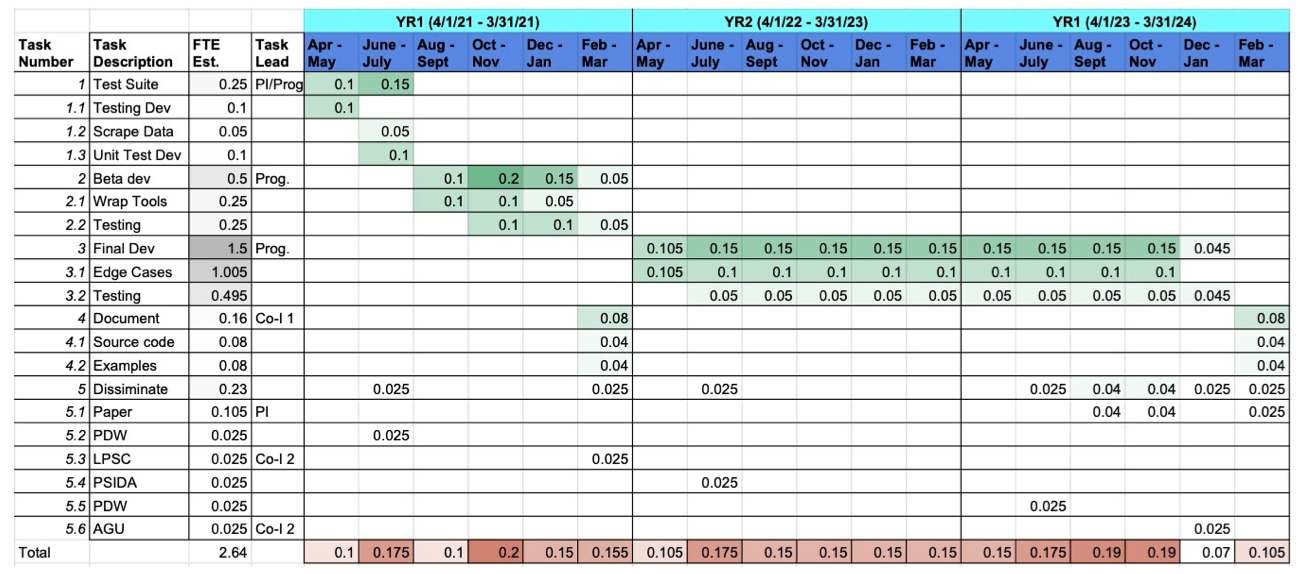
\includegraphics[width=\textwidth]{Gantt_02.png}
\centering
\end{figure}

\begin{figure}[h]
\centering
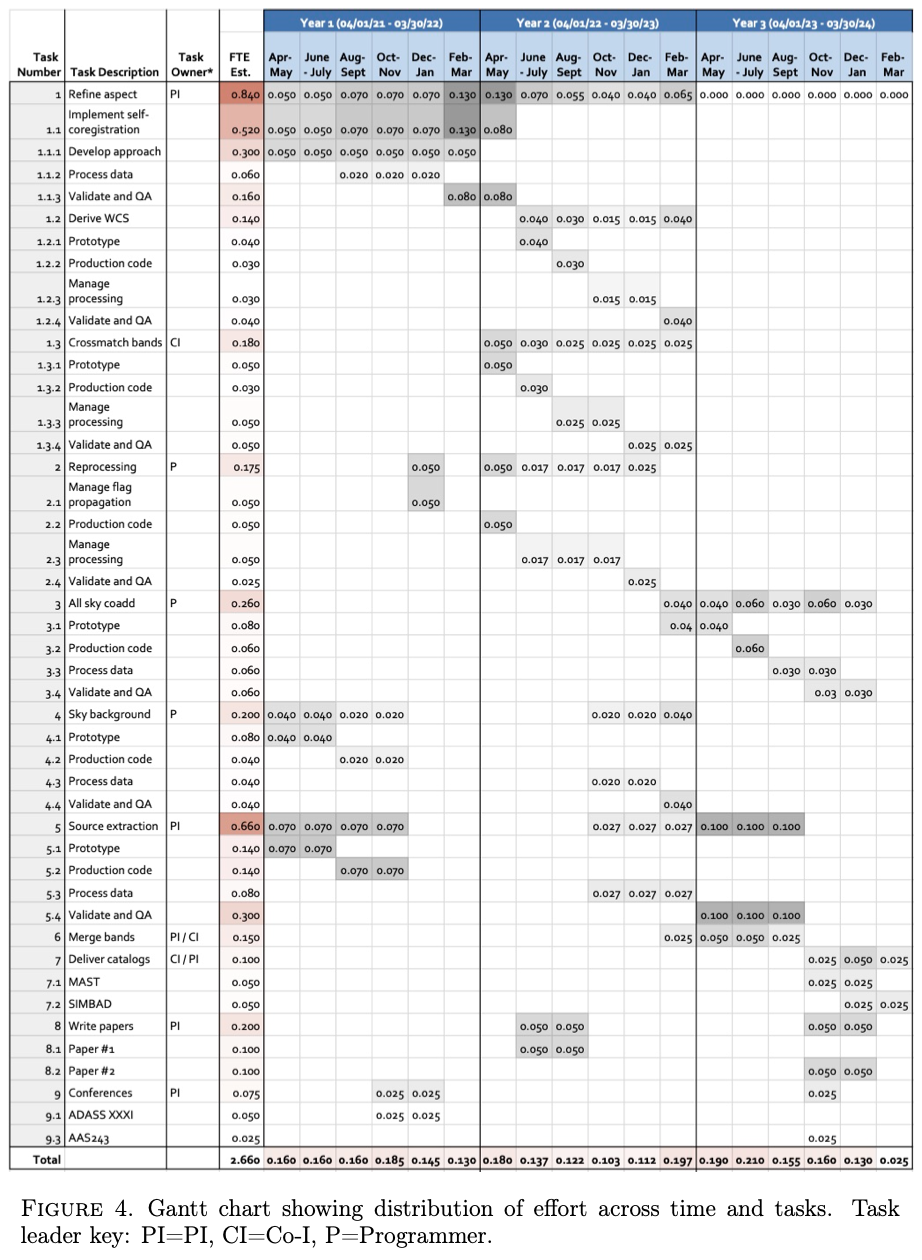
\includegraphics[width=\textwidth]{Gantt_01.png}
\centering
\end{figure}


\end{document}